\documentclass[a4paper]{article}
\usepackage{vntex}
%\usepackage[english,vietnam]{babel}
%\usepackage[utf8]{inputenc}

%\usepackage[utf8]{inputenc}
%\usepackage[francais]{babel}
\usepackage{a4wide,amssymb,epsfig,latexsym,multicol,array,hhline,fancyhdr}
\usepackage[table]{xcolor}
\usepackage{pbox}
\usepackage{amsmath}
\usepackage{lastpage}
\usepackage[lined,boxed,commentsnumbered]{algorithm2e}
\usepackage{enumerate}
\usepackage{color}
\usepackage{graphicx}							% Standard graphics package
\usepackage{array}
\usepackage{tabularx, caption}
\usepackage{multirow}
\usepackage{multicol}
\usepackage{rotating}
\usepackage{graphics}
\usepackage{geometry}
\usepackage{setspace}
\usepackage{epsfig}
\usepackage{tikz}
\usepackage{caption}
\usepackage{subcaption}
\usetikzlibrary{arrows,snakes,backgrounds}
\usepackage{hyperref}
\usepackage{titlesec}
\usepackage{float}
\usepackage{wrapfig}
\usepackage{listings}

\definecolor{dkgreen}{rgb}{0,0.6,0}
\definecolor{gray}{rgb}{0.5,0.5,0.5}
\definecolor{mauve}{rgb}{0.58,0,0.82}
 
\lstset{frame=tb,
  language=HTML,
  aboveskip=3mm,
  belowskip=3mm,
  showstringspaces=false,
  columns=flexible,
  basicstyle={\small\ttfamily},
  numbers=none,
  numberstyle=\tiny\color{gray},
  keywordstyle=\color{blue},
  commentstyle=\color{dkgreen},
  stringstyle=\color{mauve},
  breaklines=true,
  breakatwhitespace=true,
  tabsize=3
}

\restylefloat{figure}
\setcounter{secnumdepth}{4}
\fontsize{10pt}{12pt}
\titleformat{\paragraph}
{\normalfont\normalsize\bfseries}{\theparagraph}{1em}{}
\titlespacing*{\paragraph}
{0pt}{3.25ex plus 1ex minus .2ex}{1.5ex plus .2ex}

\hypersetup{urlcolor=blue,linkcolor=black,citecolor=black,colorlinks=true} 
%\usepackage{pstcol} 								% PSTricks with the standard color package

\newtheorem{theorem}{{\bf Định lý}}
\newtheorem{property}{{\bf Tính chất}}
\newtheorem{proposition}{{\bf Mệnh đề}}
\newtheorem{corollary}[proposition]{{\bf Hệ quả}}
\newtheorem{lemma}[proposition]{{\bf Bổ đề}}

\newsavebox\CBox
\def\textBF#1{\sbox\CBox{#1}\resizebox{\wd\CBox}{\ht\CBox}{\textbf{#1}}}

%\usepackage{fancyhdr}
\setlength{\headheight}{40pt}
\pagestyle{fancy}
\fancyhead{} % clear all header fields
\fancyhead[L]{
 \begin{tabular}{rl}
    \begin{picture}(25,15)(0,0)
    \put(0,-8){
\includegraphics[width=8mm, height=8mm]{hcmut.png}}
    %\put(0,-8){\epsfig{width=10mm,figure=hcmut.eps}}
   \end{picture}&
	%
\includegraphics[width=8mm, height=8mm]{hcmut.png} & %
	\begin{tabular}{l}
		\textbf{\bf \ttfamily Trường Đại Học Bách Khoa Tp.Hồ Chí Minh}\\
		\textbf{\bf \ttfamily Khoa Khoa Học và Kỹ Thuật Máy Tính}
	\end{tabular} 	
 \end{tabular}
}
\fancyhead[R]{
	\begin{tabular}{l}
		\tiny \bf \\
		\tiny \bf 
	\end{tabular}  }
\fancyfoot{} % clear all footer fields
\fancyfoot[L]{\scriptsize \ttfamily Thực tập tốt nghiệp - Niên khóa 2015-2016}
\fancyfoot[R]{\scriptsize \ttfamily Trang {\thepage}/\pageref{LastPage}}
\renewcommand{\headrulewidth}{0.3pt}
\renewcommand{\footrulewidth}{0.3pt}


%%%
\setcounter{secnumdepth}{4}
\setcounter{tocdepth}{3}
\makeatletter
\newcounter {subsubsubsection}[subsubsection]
\renewcommand\thesubsubsubsection{\thesubsubsection .\@alph\c@subsubsubsection}
\newcommand\subsubsubsection{\@startsection{subsubsubsection}{4}{\z@}%
                                     {-3.25ex\@plus -1ex \@minus -.2ex}%
                                     {1.5ex \@plus .2ex}%
                                     {\normalfont\normalsize\bfseries}}
\newcommand*\l@subsubsubsection{\@dottedtocline{3}{10.0em}{4.1em}}
\newcommand*{\subsubsubsectionmark}[1]{}
\makeatother


\begin{document}

\begin{titlepage}
\begin{center}
ĐẠI HỌC QUỐC GIA THÀNH PHỐ HỒ CHÍ MINH \\
TRƯỜNG ĐẠI HỌC BÁCH KHOA \\
KHOA KHOA HỌC VÀ KỸ THUẬT MÁY TÍNH 
\end{center}

\vspace{1cm}

\begin{figure}[h!]
\begin{center}

\includegraphics[width=3cm]{hcmut.png}
\end{center}
\end{figure}

\vspace{1cm}


\begin{center}
\begin{tabular}{c}
\multicolumn{1}{l}{\textbf{{\Large THỰC TẬP TỐT NGHIỆP}}}\\
~~\\
\hline
\\
\multicolumn{1}{l}{\textbf{{\Large Đề tài 126}}}\\
\\
\textBF{\Huge Xây dựng nền tảng và tiêu chuẩn}\\
\textBF{\Huge tương tác 2 chiều giữa chính phủ điện tử }\\
\textBF{\Huge với thiết bị di động của người dân }\\
\textBF{\Huge dựa trên công nghệ Web}\\
\\
\hline
\end{tabular}
\end{center}

\vspace{2cm}

\begin{table}[h]
\begin{tabular}{rrll}
\hspace{5 cm} & GVHD: & Thầy: Lương Thế Nhân\\
\\
& Thành viên: & Võ Văn Luận & 51202065\\
& & Trần Văn Tài & 51203241\\
\end{tabular}
\end{table}

\begin{center}
{\footnotesize TP. HỒ CHÍ MINH, THÁNG 5/2016}
\end{center}
\end{titlepage}


%\thispagestyle{empty}

\section*{Tóm tắt}
\begingroup
    \fontsize{12pt}{14.4pt}\selectfont
\textit{Bài báo cáo này trình bày quá trình nghiên cứu và hiện thực đề tài "Xây dựng nền tảng và tiêu chuẩn tương tác 2 chiều giữa chính phủ điện tử với thiết bị di động củaa người dân dựa trên công nghệ Web. Mục tiêu đề tài bao gồm:
\begin{itemize}
	\item[-] Tìm hiểu các công nghệ Web và ngôn ngữ lập trình cho thiết bị di động
	\item[-] Tìm hiểu và xây dựng web service theo chuẩn Open311 cho quy trình trên
\end{itemize}
}
\endgroup

%%%%%%%%%%%%%%%%%%%%%%%%%%%%%%%%%

\newpage
\tableofcontents
\newpage
\newpage
\section{Giới thiệu đề tài}
\subsection{Tổng quan về chính phủ điện tử}
Chính phủ điện tử (CPĐT) không có một định nghĩa cụ thể nào; trên thế giới có rất nhiều khái niệm của các tổ chức khác nhau về chính phủ điện tử. Sau đây là một số định nghĩa được sử dụng phổ biến:
\begin{itemize}
	\item[•]\textbf{Theo Liên Hợp Quốc: }Chính phủ điện tử được định nghĩa là việc sử dụng Internet và mạng toàn cầu (world-wide-web) để cung cấp thông tin và các dịch vụ của chính phủ tới công dân \cite{bib1}
	\item[•]\textbf{Theo World Bank: }Chính phủ điện tử đề cập đến việc các cơ quan chính phủ sử dụng công nghệ thông tin (chẳng hạn như mạng diện rộng, mạng Internet và mạng di động) mà có khả năng chuyển đổi mối quan hệ với công dân, doanh nghiệp và với các cơ quan chính phủ khác. Những công nghệ này có thể phục vụ cho những mục đích khác nhau: cung cấp các dịch vụ tốt hơn, cải thiện sự tương tác với doanh nghiệp, tăng cường quyền lực cho công dân thông qua việc truy cập thông tin hoặc quản lý chính phủ hiệu quả hơn. Các lợi ích mang lại có thể giảm tham nhũng, nâng cao sự minh bạch, thuận tiện hơn, tăng doanh thu và/hoặc giảm chi phí \cite{bib2}
\end{itemize}
Theo cách hiểu của chúng em, chính phủ điện tử là việc áp dụng công nghệ thông tin tiên tiến vào việc giao tiếp giữa chính phủ và công dân của mình, đem lại sự nhanh chóng, tiện lợi và minh bạch trong việc cung cấp thông tin và dịch vụ đến công dân.\\
\\
Việc hiện thực hóa chính phủ điện tử đem đến rất nhiều lợi ích cho cả chính phủ lẫn công dân; nhất là trong bối cảnh hội nhập hiện nay, Internet và di động đã được phổ biến rộng rãi trong các tầng lớp người dân, hầu hết mọi người đều có một lượng kiến thức nhất định về công nghệ thông tin, giúp cho việc sử dụng và thao tác trên ứng dụng trở nên dễ dàng hơn. Trong đó có thể kể đến các lợi ích sau đây:
\begin{itemize}
	\item[•]Việc thông tin giữa chính phủ và công dân diễn ra một cách nhanh chóng và chính xác, giúp chính phủ có thể ban hành những quyết định kịp thời, giúp công dân nắm được tình hình an ninh, xã hội một cách chi tiết
	\item[•]Giảm thiểu thời gian, khối lượng công việc và chi phí của các quy trình, thủ tục hành chính, giúp việc quản lý, hoạt động của chính phủ nhanh hơn, hiệu quả hơn
	\item[•]Về phía các tổ chức, doanh nghiệp, chính phủ điện tử giúp họ làm việc một cách dễ dàng hơn bởi mọi thủ tục, quy trình đều được "số hóa", mỗi công việc được thực hiện một cách chính xác, tin cậy. Nhờ đó, tổ chức và doanh nghiệp hoạt động hiệu quả hơn, nâng cao năng lực cạnh tranh
\end{itemize}
Tuy nhiên, việc triển khai CPĐT vào thực tiễn còn gặp nhiều khó khăn và thiếu sót. Năm 2014, theo Bảng xếp hạng chính phủ điện tử (E-Government Development Index) của Liên Hợp Quốc \cite{bib3}, Việt Nam có chỉ số phát triển CPĐT là 0.4704 (đứng hạng thứ 99 trong 193 quốc gia), tuột 16 bậc so với năm 2012 (đứng hạng 83) (Hình 1). Điều này cho thấy rằng tốc độ phát triển và phổ cập chính phủ điện tử ở Việt Nam vẫn còn chậm so với thế giới và các nước trong khu vực.
\begin{center}
    \begin{figure}[htp]
    \begin{center}
     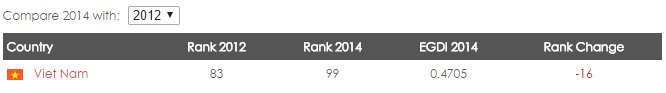
\includegraphics[scale=.85]{2014-vietnam-edgi.PNG}
    \end{center}
    \caption{Chỉ số phát triển CPĐT của Việt Nam năm 2014}
    \label{refhinh1}
    \end{figure}
\end{center}
Những khó khăn và trở ngại trong quá trình xây dựng CPĐT ở Việt Nam có thể kể đến sau đây:
\begin{itemize}
	\item[•]Cơ sở hạ tầng công nghệ thông tin ở nước ta còn yếu kém, bất cập từ các dự án công nghệ thông tin
	\item[•]Trình độ dân trí còn thấp, khó khăn trong việc sử dụng các dịch vụ của công nghệ thông tin (Web, di động,...)
	\item[•]Trình độ nhận thức và kỹ năng của cán bộ viên chức còn hạn chế, tâm lý không muốn chuyển đổi sang môi trường làm việc mới
	\item[•]Quy trình nghiệp vụ vẫn chưa ổn định, gây khó khăn cho việc xây dựng một hệ thống toàn diện
\end{itemize}
\begin{center}
    \begin{figure}[htp]
    \begin{center}
     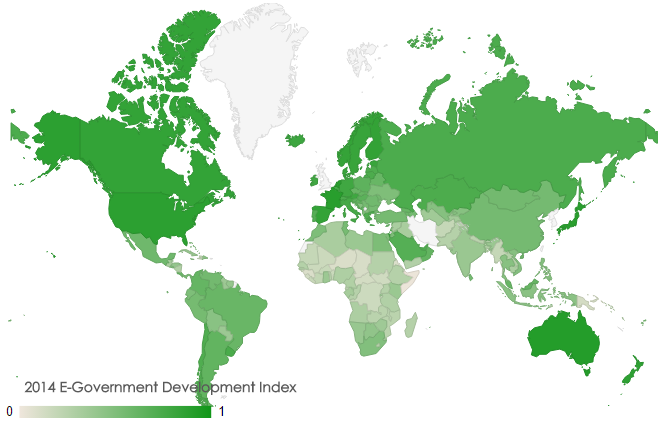
\includegraphics[scale=.8]{2014-edgi.PNG}
    \end{center}
    \caption{Chỉ số phát triển CPĐT các quốc gia năm 2014}
    \label{refhinh2}
    \end{figure}
\end{center}
Hiện nay, các dự án CPĐT đang được đẩy mạnh, nhiều cuộc tọa đàm với chủ đề công nghệ thông tin được tổ chức thường xuyên, cho thấy chính phủ ngày càng dành nhiều sự quan tâm đến việc công nghệ hóa các dịch vụ công. Ngày 14/10/2015, Chính phủ ban hành Nghị quyết số 36a/NQ-CP về Chính phủ điện tử, trong đó có một mục tiêu quan trọng là \textit{"Phấn đấu đến hết năm 2016, các bộ, ngành Trung ương có 100\% các dịch vụ công được cung cấp trực tuyến ở mức độ cho phép người sử dụng điền và gửi trực tuyến các mẫu văn bản đến cơ quan, tổ chức cung cấp dịch vụ".} Điều đó đã nêu lên được tầm quan trọng của CPĐT trong việc phát triển kinh tế, xã hội quốc gia. 
\subsection{Chi tiết về đề tài}
Nhiệm vụ chủ yếu của đề tài là xây dựng kênh tương tác 2 chiều giữa chính phủ và người dân tại địa bàn Thành phố Hồ Chí Minh, dựa trên 2 nền tảng là Web và di động. Trong đó, tương tác 2 chiều trong phạm vi của đề tài có nghĩa là:
\begin{itemize}
     \item[•]Ứng dụng cho phép người dân phản ánh các sự cố (điện, nước, giao thông,...) cho các cơ quan chức năng để họ có thể khắc phục kịp thời; duyệt xem và bình luận các phản ánh trước đó; xem các thông báo mới của chính phủ 
     \item[•]Chính phủ có thể thông báo đến người dân các tin tức về đời sống, xã hội (lịch cúp điện, công trình giao thông đang thi công,...); thu thập góp ý từ phía công dân, đưa mỗi phản ánh về các cơ quan chức năng chuyên biệt để giải quyết vấn đề, phản hồi nhanh chóng cho người dân
\end{itemize}
Môi trường làm việc:
\begin{itemize}
	\item[•]Hệ quản trị cơ sở dữ liệu: MySQL Server
	\item[•]Ngôn ngữ lập trình: Java, AngularJS, HTML, CSS, Javascript
	\item[•]Công cụ lập trình: NetBeans, Android Studio, Sublime Text
	\item[•]Hệ thống quản lý mã nguồn: GitHub
\end{itemize}
%%%%%%%%%%%%%%%%%%%%%%%%%%%%%%%%%
\section{Các dự án tương tự}
\subsection{Trên thế giới}
\subsubsection{New York}
\url{Nyc.gov} là tên miền trang web CPĐT của thành phố New York. Hiện có hơn 30,000 trang nội dung và 100 dịch vụ giao dịch online trên trang web này. Giao dịch online bao gồm: mua vé đậu xe, theo dõi tình trạng bất động sản, nhận các chứng chỉ hoặc giấy phép từ chính phủ, hoặc đơn giản hơn là xem lịch đổ rác ở khu phố đang sống… Cổng CPĐT của thành phố cập nhật các thông tin khẩn cấp và thông báo đến toàn thể người dân thành phố rất dễ dàng.
\newpage
\begin{center}
    \begin{figure}[t]
    \begin{center}
     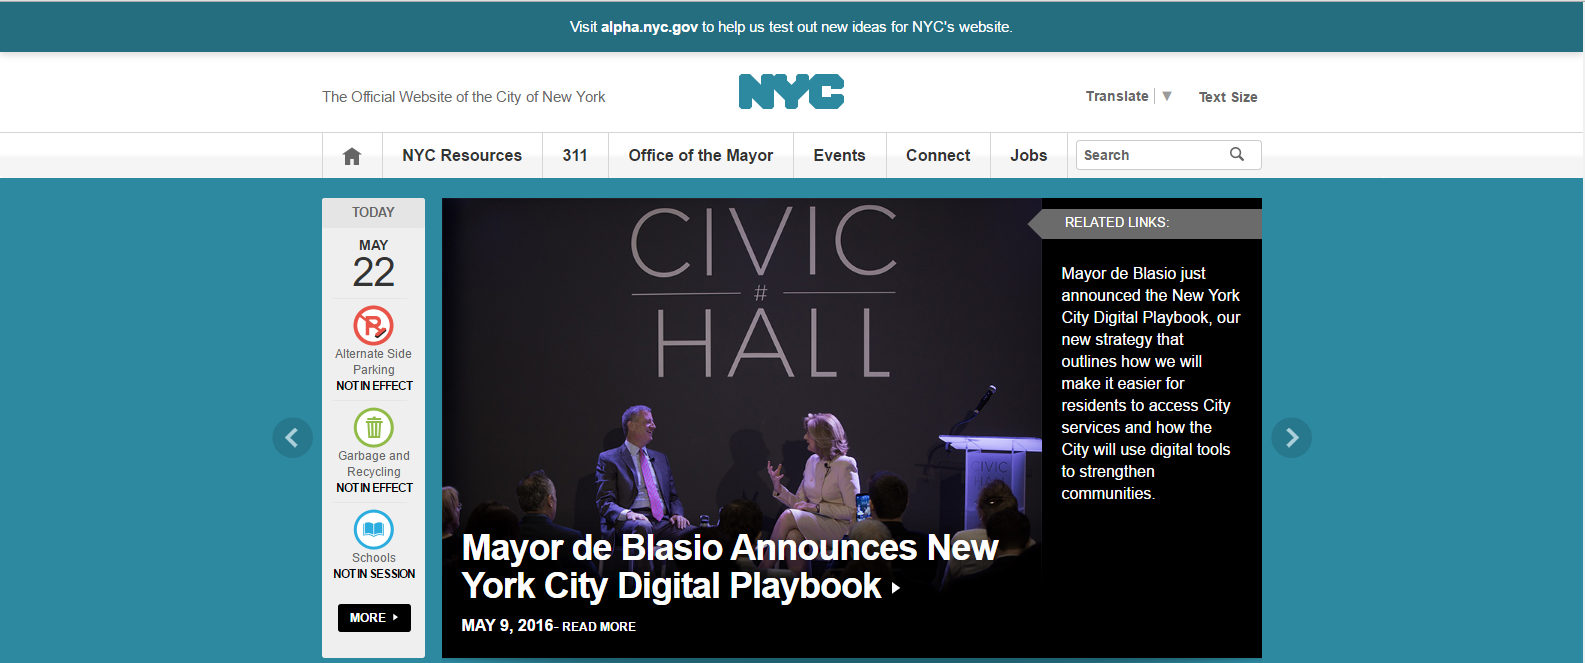
\includegraphics[scale=.34]{newyork.PNG}
    \end{center}
    \caption{Trang web CPĐT \url{Nyc.gov} của thành phố New York}
    \label{refhinh2}
    \end{figure}
\end{center}
Người dân có thể dễ dàng gửi phản ánh về vấn đề xung quanh như: tiếng ồn, đậu xe không đúng chỗ, xả rác, mất trật tự an ninh... đến chính quyền thành phố từ trang web \url{http://www1.nyc.gov/311/}. Chính quyền sẽ phản hồi và nhanh chóng giải quyết vấn đề. Ngoài ra, người dân cũng có thể thanh toán các dịch vụ công cộng như: vé đậu xe, vé phạt tốc độ, vượt đèn đỏ,... trên trang web này.
\begin{center}
    \begin{figure}[h]
    \begin{center}
     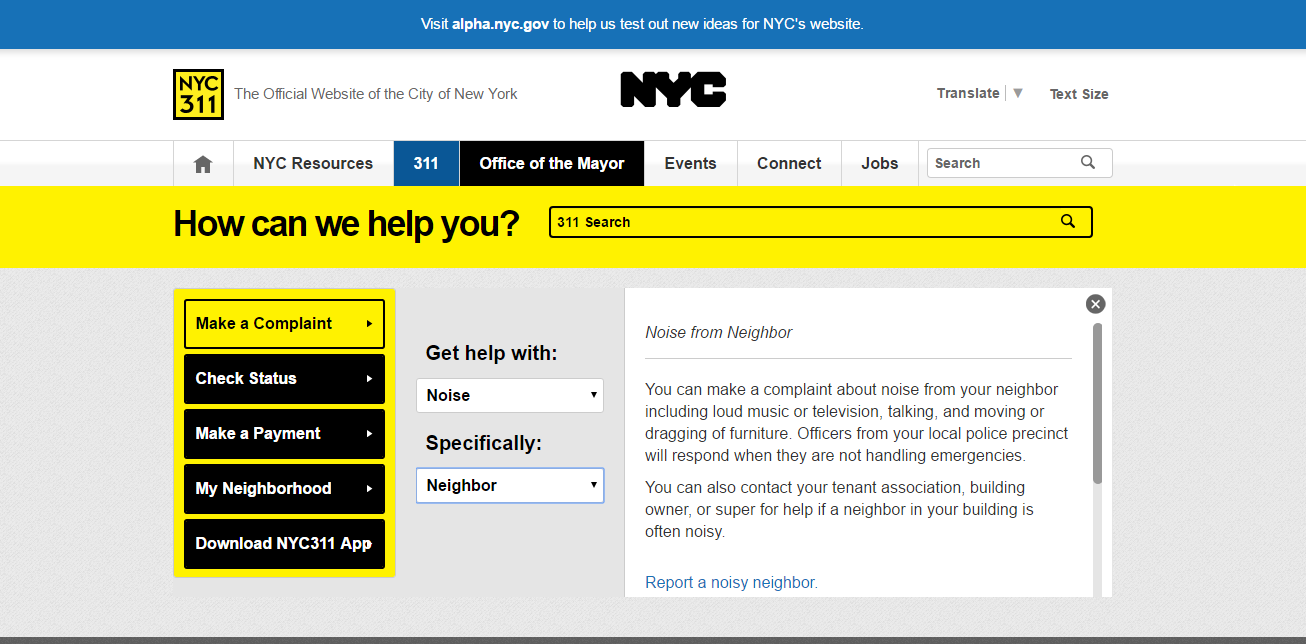
\includegraphics[scale=.41]{newyork_complaint.PNG}
    \end{center}
    \caption{Gửi lời phàn nàn đến chính quyền}
    \label{refhinh2}
    \end{figure}
\end{center}
\newpage
\begin{center}
    \begin{figure}[h]
    \begin{center}
     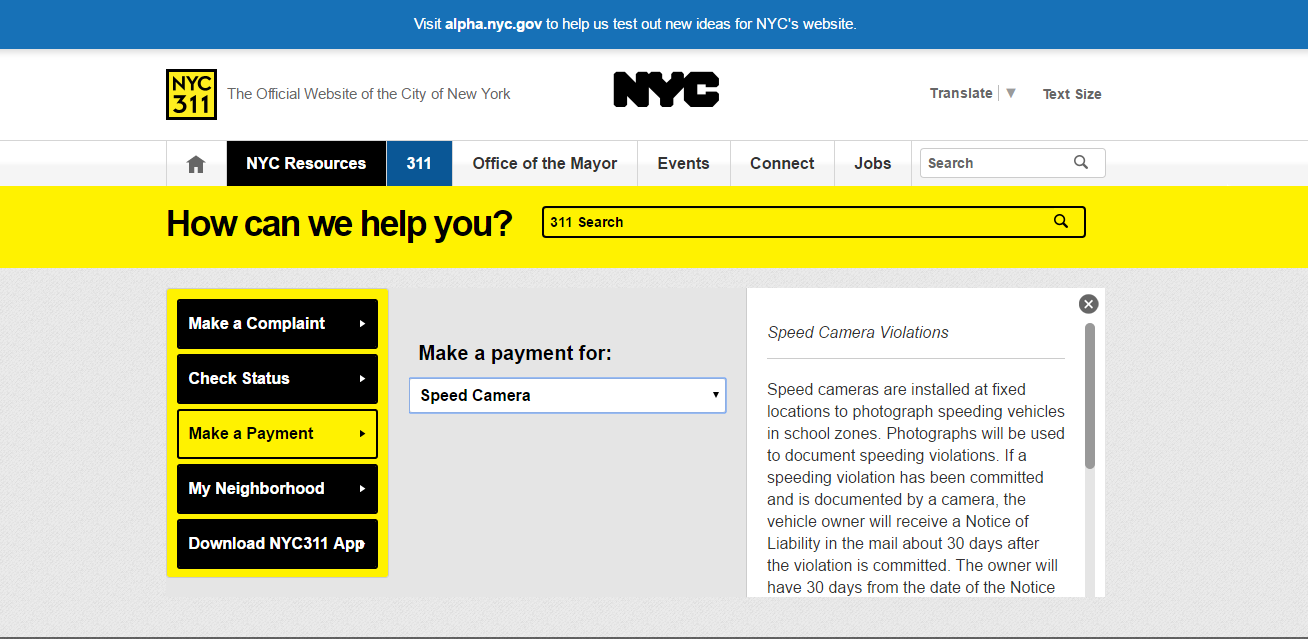
\includegraphics[scale=.4]{newyork_payment.PNG}
    \end{center}
    \caption{Người dân thanh toán phí công cộng}
    \label{refhinh2}
    \end{figure}
\end{center}
Không chỉ phát triển trên nền tảng web, CPĐT ở New York còn phát triển trên các ứng dụng điện thoại di động, đặc biệt là trên hệ điều hành Android và iPhone (Hình 6). Với sự tiện ích và gắn bó bên cạnh người dùng của điện thoại di động, người dân có thể gửi yêu cầu đến chính quyền thành phố nhanh chóng và kịp thời.\\
\\
Từ sau chấn động 11/9, thành phố New York càng tập trung phát triển CPĐT để tạo ra kênh thông tin cho người dân thành phố trong các tình huống khẩn cấp. Hiện nay, New York là một trong các thành phố phát triển nhất thế giới về CPĐT.
\begin{figure}[h]
\centering
\begin{subfigure}{.5\textwidth}
  \centering
  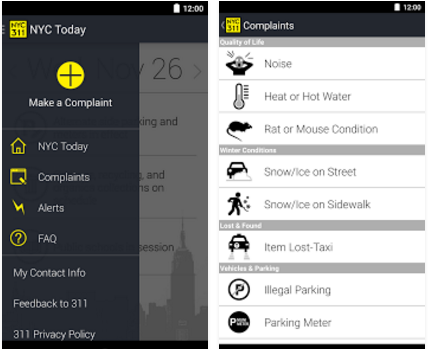
\includegraphics[width=0.9\linewidth]{newyork_android.PNG}
  \caption{NYC android app}
\end{subfigure}%
\begin{subfigure}{.47\textwidth}
  \centering
  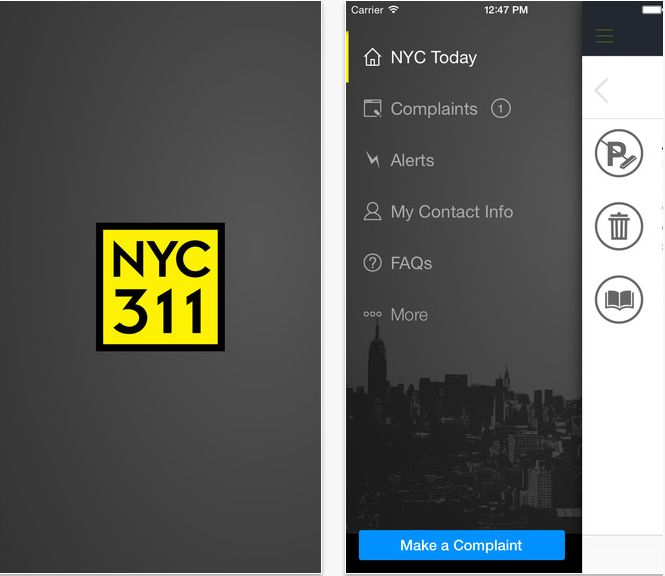
\includegraphics[width=0.9\linewidth]{newyork_iphones.PNG}
  \caption{NYC iPhone app}
  \label{fig:sub2}
\end{subfigure}
\caption{Ứng dụng CPĐT của New York trên hệ điều hành Android và iPhone}
\end{figure}
\subsubsection{Singapore}
Là một trong những quốc gia tiên phong về CPĐT, Singapore bắt tay vào CPĐT với các kế hoạch công nghệ thông tin tổng thể ở cấp quốc gia và tin học hóa quản lý hành chính kể từ những năm 80 của thế kỷ 20. Singapore nổi tiếng về mô hình "một cửa" trong dịch vụ công và đã triển khai thành công CPĐT. Singapore rất nỗ lực trong việc đầu tư phát triển CPĐT và đã đạt được nhiều thành tựu quan trọng, xếp hạng cao trong các đánh giá toàn cầu về CPĐT:
\begin{itemize}
	\item[-]Trong cuộc khảo sát của Liên Hiệp Quốc về CPĐT:
	\begin{itemize}
	\item[•]Đứng thứ 2 về chỉ số tham gia CPĐT
	\item[•]Đứng thứ 10 về chỉ số phát triển CPĐT
	\end{itemize}
	\item[-]Đứng thứ nhất trong cuộc khảo sát hằng năm về CPĐT của trường đại học Waseda
\end{itemize}
CPĐT ở Singapore nhận được sự tin tưởng của người dân từ khi được triển khai. 93\% người dân hài lòng và cảm thấy có ích về những thông tin được đăng trên trang web của chính phủ, 94\% bằng lòng với chất lượng dịch vụ CPĐT.
Hiện nay, có 4 cổng CPĐT và hơn 400 websites chi nhánh giải quyết từng vấn đề cụ thể ở Singapore. Không chỉ vậy, \url{https://www.ecitizen.gov.sg} là cổng CPĐT riêng để người dân có thể truy cập các thông tin và dịch vụ điện tử của chính phủ.	
\begin{center}
    \begin{figure}[h]
    \begin{center}
     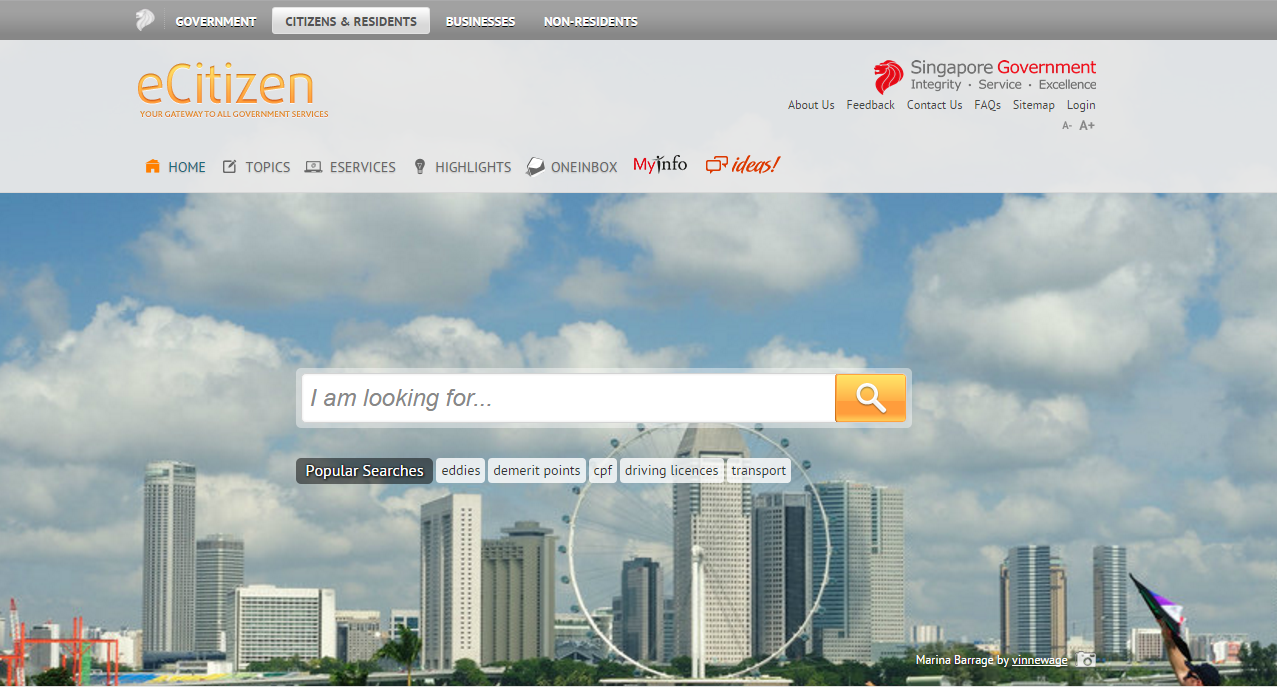
\includegraphics[scale=.4]{singapore.PNG}
    \end{center}
    \caption{Trang web CPĐT \url{ecitizen.gov.sg} của thành phố Singapore}
    \label{refhinh2}
    \end{figure}
\end{center}
Người dân dễ dàng truy cập vào tất cả thông tin và dịch vụ chính phủ. Đồng thời, trang \url{ecitizen.gov.sg} cũng liên kết đến các websites chi nhánh để cung cấp chi tiết thông tin hay dịch vụ người dân cần. 
Ngoài ra, CPĐT ở Singapore còn có hệ thống cung cấp giấy phép, chứng chỉ kinh doạnh điện tử, mang lại nhiều lợi ích về thời gian và chi phí:
	\begin{itemize}
	\item[•]Tự động cập nhật tình trạng qua tin nhắn hoặc email
	\item[•]Giảm 90\% thời gian làm thủ tục
	\item[•]Giảm 50\% thời gian nhập dữ liệu  
	\end{itemize}
\subsection{Tại Việt Nam}
\subsubsection{Thành phố Hồ Chí Minh}	
Trang web \url{hochiminhcity.gov.vn} là cổng thông tin chính phủ điện tử ở tại Thành phố Hồ Chí Minh. Trang web với hơn 7000 lượt truy cập mỗi ngày, cung cấp các tin tức, hoạt động nổi bật của thành phố, các văn bản chỉ đạo điều hành, văn bản quy phạm pháp luật, các báo cáo thống kê và tình hình kinh tế - xã hội.\\
\\
Ngoài ra trang web còn cho phép công dân gửi góp ý về các quy định, thủ tục hành chính, những vướng mắc cụ thể trong việc thực hiện các quy định hành chính; người dân cũng có thể đề xuất với chính quyền các phương án xử lý những phản ánh nêu trên hoặc có sáng kiến ban hành mới quy định hành chính liên quan đến hoạt động kinh doanh, đời sống nhân dân.
\begin{center}
    \begin{figure}[h]
    \begin{center}
     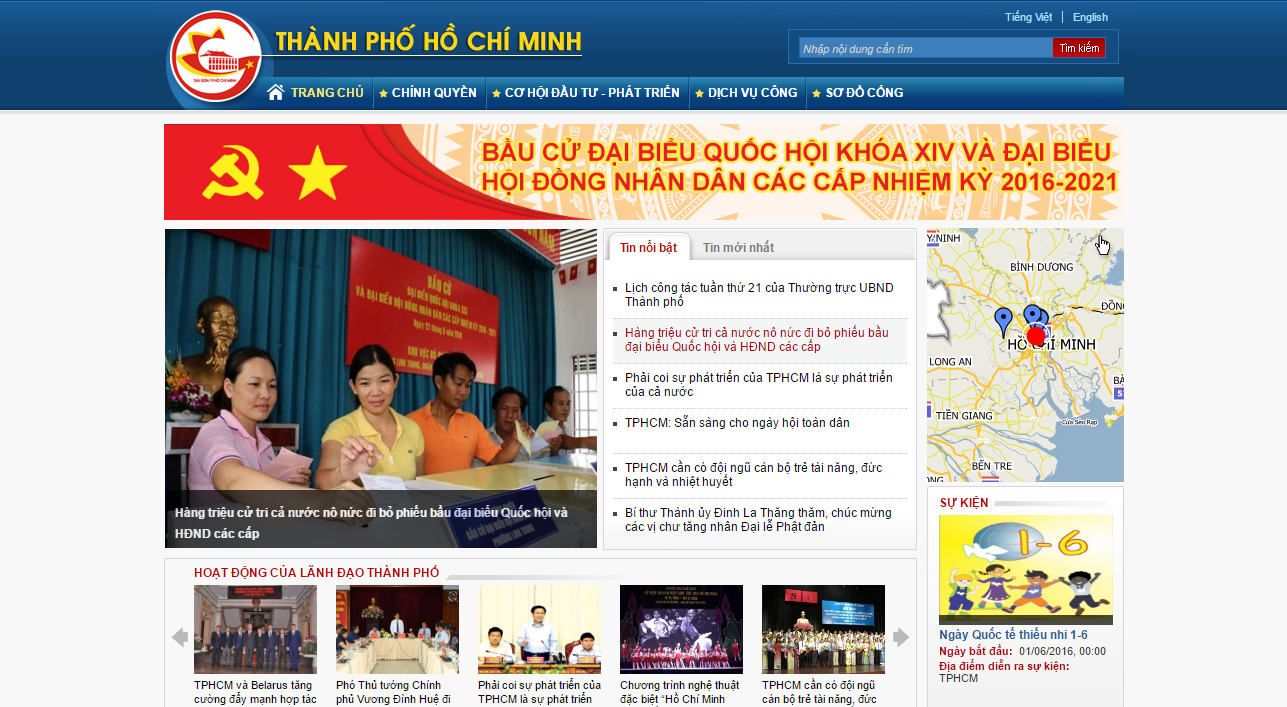
\includegraphics[scale=.4]{egov-tphcm.PNG}
    \end{center}
    \caption{Trang web CPĐT \url{hochiminhcity.gov.vn} của thành phố Hồ Chí Minh}
    \label{refhinh7}
    \end{figure}
\end{center}
Tuy nhiên, trang web vẫn còn nhiều bất cập và thiếu sót, trang góp ý (Hình 9) còn đơn giản, chưa đi sâu vào chi tiết các mảng, chưa phân hóa ra thành các mục chuyên biệt rõ ràng; trang web không hiển thị cho người xem các phản ánh trước đó, do đó người dân không biết được tình trạng cũng như các cơ quan chức năng nào đang xử lý phản ánh, góp ý, không tạo được kênh tương tác giữa chính phủ và công dân.
\newpage
\begin{center}
    \begin{figure}[h]
    \begin{center}
     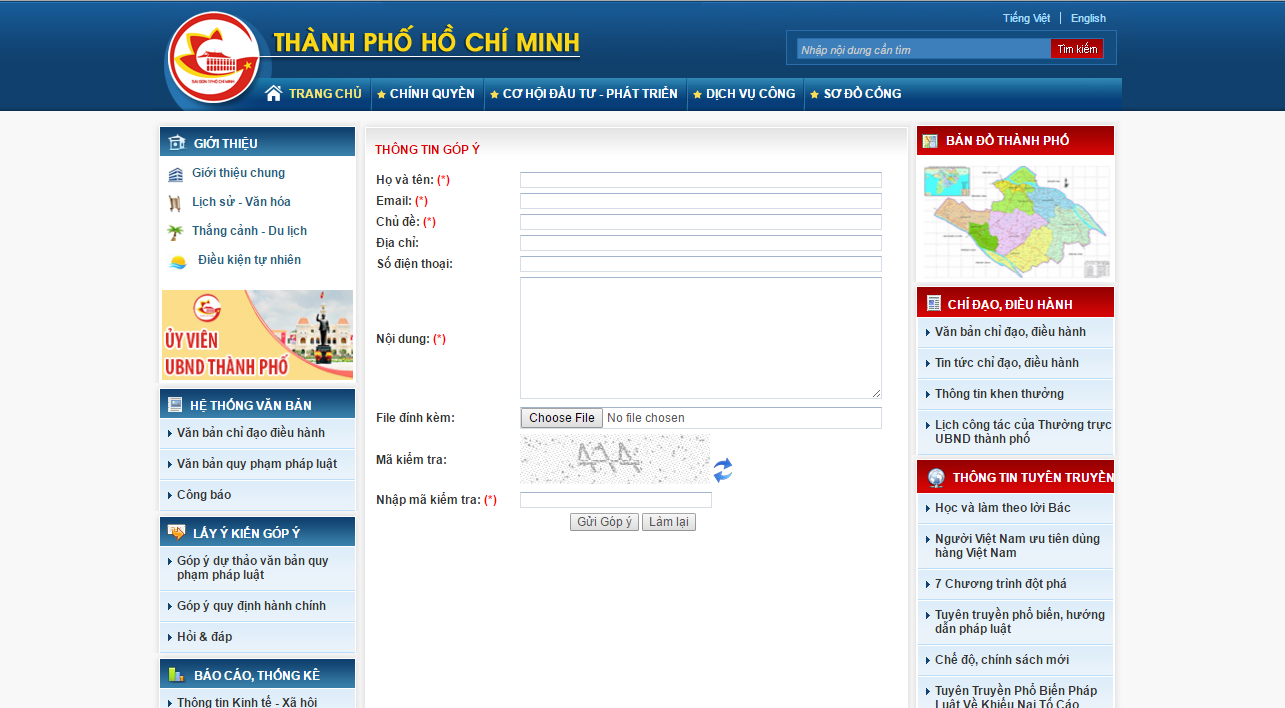
\includegraphics[scale=.36]{gopy-tphcm.PNG}
    \end{center}
    \caption{Trang góp ý của \url{hochiminhcity.gov.vn}}
    \label{refhinh7}
    \end{figure}
\end{center}
\subsubsection{Thành phố Đà Nẵng}
Vào tháng 8/2014, ông Phạm Kim Sơn, Giám đốc Sở Thông tin \& Truyền thông công bố chia sẻ miễn phí nền tảng Chính phú điện tử \textbf{eGov Framework} cho các địa phương. \textbf{eGov Framework} là giải pháp nền tảng về Chính phủ điện tử được chuyển giao từ Chính phủ Hàn Quốc.\\
\\
Cùng với sự tư vấn của các chuyên gia ở Hoa Kỳ, Đà Nẵng đã phối hợp phát triển thêm nền tảng Chính phủ điện tử phù hợp với điều kiện địa phương trong suốt 2 năm với chi phí bỏ ra khoảng 630.000 USD, cho ra đời hệ thống thông tin chính quyền điện tử Thành phố Đà Nẵng tại đường dẫn \url{egov.danang.gov.vn}. 
\begin{center}
    \begin{figure}[h]
    \begin{center}
     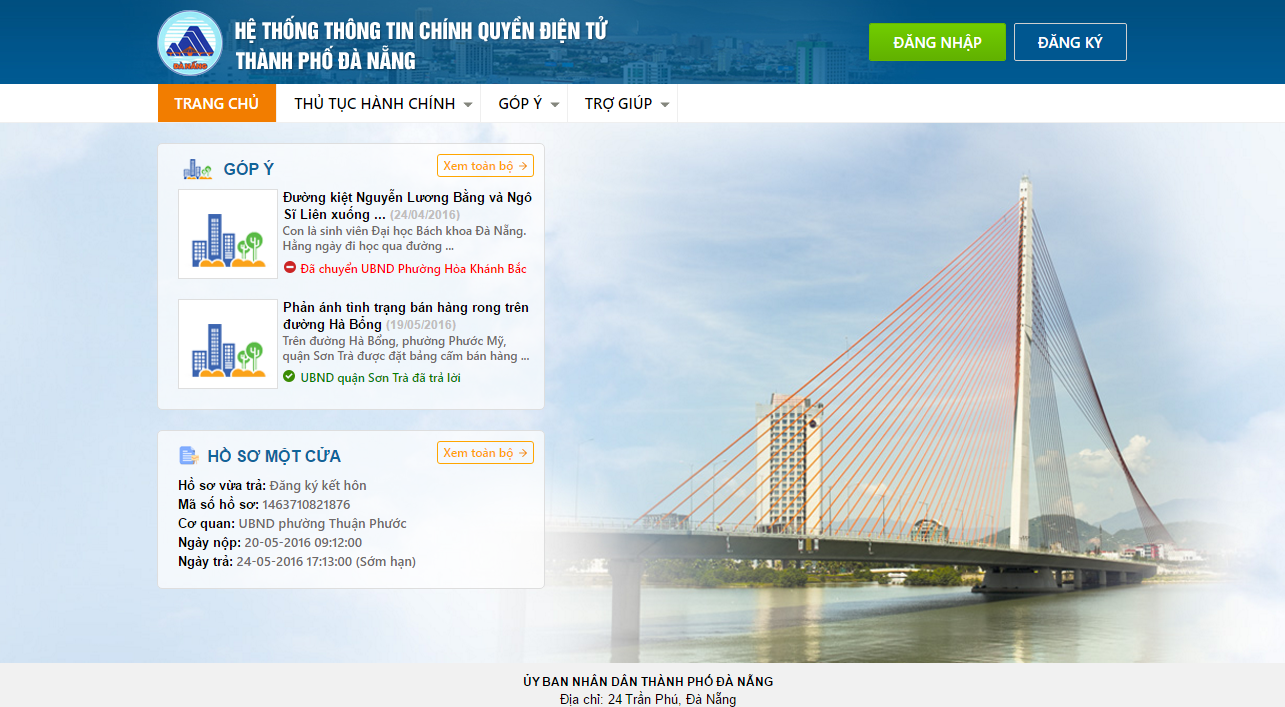
\includegraphics[scale=.36]{egov-danang.PNG}
    \end{center}
    \caption{Trang web CPĐT \url{egov.danang.gov.vn} của Thành phố Đà Nẵng}
    \label{refhinh7}
    \end{figure}
\end{center}
Trang web cho phép công dân, doanh nghiệp sau khi đăng nhập bằng tài khoản đã được đăng ký và xác thực bởi cơ quan nhà nước có thể thực hiện các dịch vụ hành chính công một cách đơn giản và thuận tiện. Công dân, doanh nghiệp quản lý được hồ sơ cá nhân (thông tin cá nhân, giấy tờ số) và toàn bộ các giao dịch với cơ quan nhà nước thông qua việc nộp, theo dõi tình hình xử lý và nhận kết quả xử lý hồ sơ thực hiện dịch vụ hành chính công trực tiếp tại bộ phận một cửa hoặc trực tuyến tại Hệ thống thông tin chính quyền điện tử TP Đà Nẵng. Ngoài ra, công dân và doanh nghiệp còn dễ dàng khai thác các dịch vụ công.\\
\\
Cán bộ sử dụng Hệ thống thông tin chính quyền điện tử để tiếp nhận hồ sơ trực tuyến, tiếp nhận hồ sơ trực tiếp, luân chuyển và xử lý hồ sơ, trả kết quả hồ sơ và thực hiện thống kê, báo cáo tùy theo vai trò được phân công.
\begin{center}
    \begin{figure}[h]
    \begin{center}
     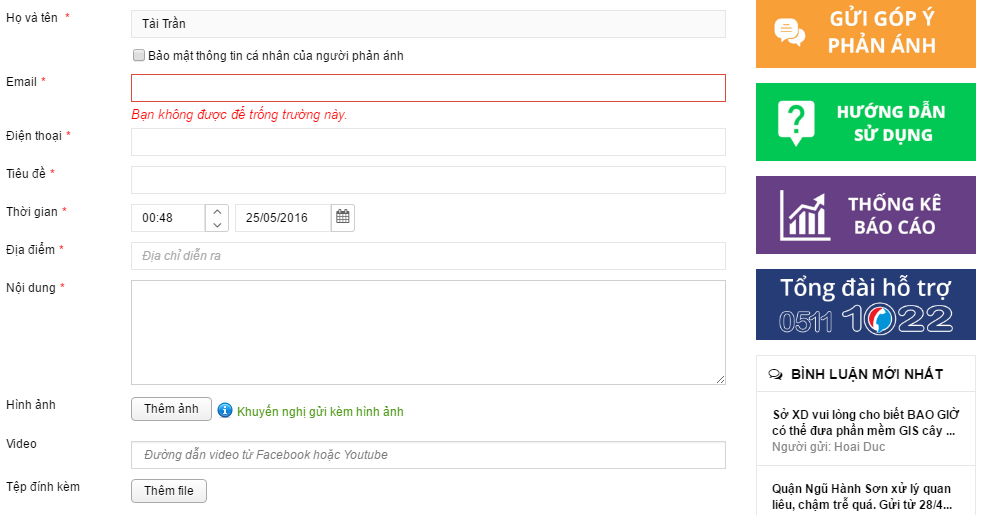
\includegraphics[scale=.55]{gopy-danang.PNG}
    \end{center}
    \caption{Trang góp ý của \url{egov.danang.gov.vn}}
    \label{refhinh7}
    \end{figure}
\end{center}
Không những thế, chính quyền Đà Nẵng còn mở thêm cổng thông tin \textit{"Quản lý đô thị Đà Nẵng: Tiện nghi - Xanh - Sạch - Đẹp"} trên mạng xã hội Facebook tiếp nhận các phản ánh của người dân về các vấn đề an ninh đô thị, môi trường, v.v\\
\\
Ngoài ra, Đà Nẵng còn cung cấp \textit{"Tổng đài dịch vụ công 1022"} trên mạng xã hội Zalo (Hình 12). Tổng đài chính thức đi vào hoạt động ngày 15/12/2015, cung cấp các tin tức nổi bật hàng ngày tại Đà Nẵng, cho phép người dân tra cứu hành trình xe buýt, tình trạng nộp hồ sơ đăng ký kinh doanh. Trong tương lai, Tổng đài trên Zalo còn dự kiến cung cấp nhiều loại thông tin hữu ích khác tới người dân như tình hình bão lũ và hướng dẫn phòng tránh; lịch tiếp dân; lịch cắt điện, cắt nước; văn bản, chính sách mới của thành phố, điểm thi tốt nghiệp THCS, THPT, Đại học…

\newpage
\begin{figure}[h]
\centering
\begin{subfigure}{.5\textwidth}
  \centering
  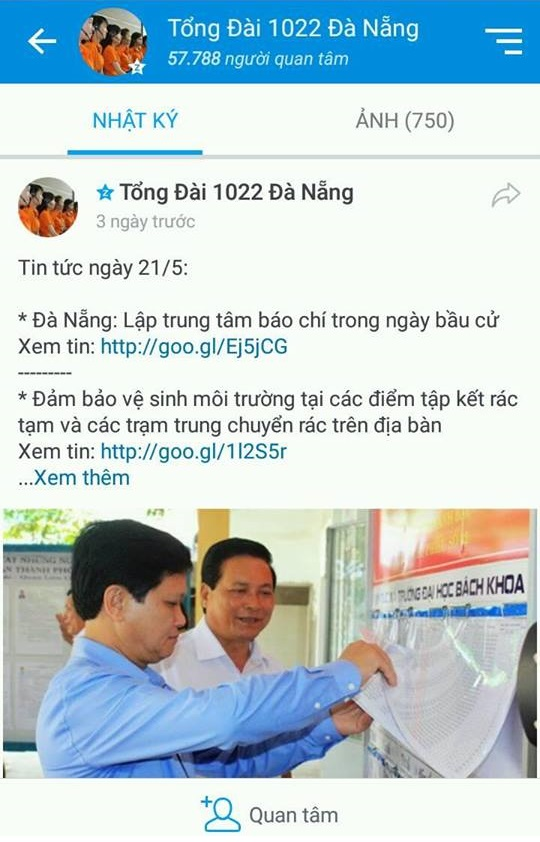
\includegraphics[width=0.7\linewidth]{zalo-danang-1.jpg}
  \caption{}
\end{subfigure}%
\begin{subfigure}{.5\textwidth}
  \centering
  
\includegraphics[width=0.7\linewidth]{zalo-danang-2.jpg}
  \caption{}
  \label{fig:sub2}
\end{subfigure}
\caption{Ứng dụng CPĐT của Đà Nẵng trên Zalo}
\end{figure}
Việc sử dụng các mạng xã hội như Facebook và Zalo vào mô hình CPĐT giúp cho thông tin có độ phủ lớn, đến với người dân rất nhanh, phản ứng của chính quyền kịp thời. Điều này cho thấy Đà Nẵng đã dẫn đầu xu hướng CPĐT tại Việt Nam, tiên phong trong việc triển khai chính phủ điện tử trên nền tảng OTT, đón đầu cả xu thế sử dụng điện thoại di động ngày càng phổ biến trong xã hội.
%%%%%%%%%%%%%%%%%%%%%%%%%%%%%%%%%
\section{Kiến thức nền}
\subsection{Open311}
Thách thức của các chính phủ hiện nay là việc tiếp nhận hàng loạt các yêu cầu dịch vụ từ phía người dân thông qua nhiều kênh và cách thức khác nhau (điện thoại, website, email, ứng dụng di động, ...). Bên cạnh đó chính phủ cũng phải kiểm soát được các chi phí phát sinh khi các kênh tương tác được phát triển mỗi ngày. Một câu trả lời khả thi cho các vấn đề trên là công nghệ có tên Open311
\subsubsection{Giới thiệu và định nghĩa}
Hiện nay, dựa vào sự phát triển của CNTT người dân có thể gửi những yêu cầu, nguyện vọng của bản thân đến chính quyền thông qua email. Một email phản ánh việc một miếng đá lát trên đường Nguyễn Huệ bị vỡ được gửi đến một nhân viên chính quyền. Người này sẽ lấy đoạn email và lưu vào cơ sở dữ liệu, sau đó gửi đến cơ quan chức năng có trách nhiệm giải quyết vấn đề này.\\
\\
Thay vì vậy, nếu báo cáo về miếng đá bị vỡ được gửi trực tiếp từ người dân đến ban ngành quản lý việc sửa chữa mặt đường, sẽ giảm thiểu rất nhiều chi phí quản lý. Đồng thời, chính quyền cần phải thông báo người dân khi vấn đề đã được giải quyết. Vấn đề bức thiết là phải tạo ra một giao thức để người dân có thể gửi yêu cầu dịch vụ tới chính quyền, và nhận thông báo về tiến trình giải quyết vấn đề đó. Ý tưởng này đã được nhóm kỹ sư tại OpenPlans (một công ty CNTT ở Mỹ) quan tâm và họ đã xây dựng một dự án có tên Open311 vào năm 2009.\\
\newpage
Open311 là một phương thức mà người dân có thể thông qua nó để gửi các yêu cầu dịch vụ vào danh sách các việc cần làm của chính quyền địa phương, và là cách thức để người dân biết được tiến trình xử lý của chính quyền nhanh chóng và dễ dàng.
\subsubsection{GeoReport v2}
GeoReport v2 là một API của Open311 để xây dựng những ứng dụng có thể xem và phản ánh vấn đề đến chính quyền.
Một số thành phố đang sử dụng API GeoReport v2:
\begin{itemize}
    \item[•]Helsinki, Finland
	\item[•]Bonn, Germany
	\item[•]Lamía, Greece
	\item[•]Chicago, Illinois
	\item[•]Toronto, Ontario
	\item[•]San Francisco, California
	\item[•]Washington D.C
	\item[•]Boston, Massachusetts
	\item[•]Baltimore, Maryland
	\item[•]Bloomington, Indiana
	\item[•]New Haven, Connecticut
\end{itemize}
Tiếp theo, nhóm xin giới thiệu một số thông tin cơ bản về API GeoReport v2
\paragraph*{Định dạng ngày/giờ}
Mọi ô dữ liệu kiểu ngày/giờ phải định dạng theo một tập con chung của chuẩn ISO 8601. Thông tin về múi giờ phải có trong định dạng.\\
\\
Ví dụ: 1994-11-05T08:15:30-05:00 nghĩa là  November 5, 1994, 8:15:30 am, US Eastern Standard Time

\paragraph*{Mã hóa}
GeoReport yêu cầu sử dụng UTF-8. Mọi kí tự trả về ở dạng XML, JSON, hoặc bất kỳ một định dạng khác phải được mã hóa dưới dạng UTF-8. Những HTTP headers phải thêm thuộc tính encoding = "UTF-8". Mọi kí tự nhận được bởi dịch vụ từ client sẽ được đưa về UTF-8 và được giải mã một cách phù hợp. 
\paragraph*{Hỗ trợ định dạng}
Định dạng có thể sử dụng trong GeoReport v2 là XML hoặc JSON.
HTTP content-type headers của mỗi định dạng sẽ là: \\
\\
\textbf{XML}: Content-Type: text/xml; charset=utf-8\\
\textbf{JSON}: Content-Type: application/json; charset=utf-8
\paragraph*{Các phương thức API}
\begin{itemize}
	\item \textbf{GET Service List} cung cấp danh sách các yêu cầu dịch vụ và các mã code tương ứng của từng loại dịch vụ.
	\item \textbf{GET Service Definition} định nghĩa các thuộc tính tương ứng với một mã dịch vụ.
	\item \textbf{POST Service Request} gửi một yêu cầu dịch vụ từ client lên server.
	\item \textbf{GET Service Request} lấy thông tin về tiến trình hiện tại của yêu cầu: đang xem xét hoặc đã giải quyết...
	\item \textbf{GET Service Requests} lấy thông tin của nhiều yêu cầu dịch vụ.
\end{itemize}
\paragraph*{Các thuộc tính cần có trong cơ sở dữ liệu}
Với chuẩn GeoReport v2, một số thuộc tính sau bắt buộc phải có trong cơ sở dữ liệu:
\begin{itemize}
	\item \textbf{jurisdiction\_id} là định danh độc nhất của từng thành phố, dùng để phân biệt các thành phố trong trường hợp hiện thực cho nhiều thành phố.
	\item \textbf{service\_code}: Mã code quy định loại dịch vụ
	\item \textbf{service\_name}: Tên có thể đọc được của dịch vụ
	\item \textbf{description}: Mô tả ngắn gọn về dịch vụ, yêu cầu
	\item \textbf{lat}: Vĩ độ vị trí xảy ra vấn đề cần gửi báo cáo, yêu cầu lên chính quyền
	\item \textbf{long}: Kinh độ vị trí xảy ra vấn đề cần gửi báo cáo, yêu cầu lên chính quyền
	\item \textbf{address}: người dùng nhập địa chỉ, hoặc mô tả địa điểm
	\item \textbf{address\_id}: ID của địa chỉ
	\item \textbf{status}: tình trạng hiện tại của yêu cầu(đang xem xét, đã giải quyết)
	\item \textbf{agency\_responsible}: cơ quan chịu trách nhiệm giải quyết yêu cầu
	\item \textbf{requested\_datetime}: thời điểm yêu cầu được gửi
	\item \textbf{updated\_datetime}: thời điểm yêu cầu được cập nhật
	\item \textbf{expected\_datetime}: dự tính yêu cầu sẽ được giải quyết xong vào thời điểm này
	\item \textbf{email}: địa chỉ email của người gửi yêu cầu
	\item \textbf{device\_id}: ID của thiết bị gửi yêu cầu
	\item \textbf{account\_id}: ID của tài khoản người dùng gửi yêu cầu
	\item \textbf{first\_name}: tên của người gửi yêu cầu
	\item \textbf{last\_name}: họ của người gửi yêu cầu
	\item \textbf{phone}: số điện thoại của người gửi yêu cầu
	\item \textbf{media\_url}: đường dẫn đến ảnh, clip... mô tả về yêu cầu
\end{itemize}
\subsection{RESTful Web Service}
REST (Representational State Transfer) định nghĩa các quy tắc kiến trúc thiết kế Web services chú trọng vào tài nguyên hệ thống, các tài nguyên này được chuyển tải thông qua giao thức HTTP. REST được giới thiệu lần đầu tiên vào năm 2000 bởi Roy Fielding trong luận án của ông \textit{"Architectural Styles and the Design of Network-based Software Architectures"}.\\
\\
Việc cụ thể hóa một Web service REST sẽ tuân thủ theo bốn nguyên tắc thiết kế sau: \cite{bib11}
 \begin{itemize}
 	\item[•]Sử dụng các phương thức HTTP một cách rõ ràng
	\item[•]Phi trạng thái
	\item[•]URIs hiển thị theo dạng cấu trúc thư mục
	\item[•]Biểu diễn tài nguyên 
 \end{itemize}
\subsubsection{Sử dụng các phương thức HTTP một cách rõ ràng}
Một đặc tính quan trọng của dịch Web service RESTful là sử dụng một cách rõ ràng các phương thức HTTP theo cách một giao thức được xác định bởi RFC 2616. Ví dụ HTTP GET được xác định như là một phương thức sinh ra số liệu được sử dụng có chủ đích bởi các ứng dụng người dùng để thu thập tài nguyên, dữ liệu từ một máy chủ, hoặc thực thi một truy vấn mà máy chủ sẽ tìm kiếm và phản hồi cùng với một gói thông tin tương thích.\\
\\
Dưới đây là các phương thức HTTP được sử dụng phổ biến trong kiến trúc REST:
\begin{itemize}
\item[•]\textbf{GET} - truy xuất một tài nguyên 
\item[•]\textbf{PUT} - thay đổi trạng thái một tài nguyên hoặc để cập nhật nó
\item[•]\textbf{POST} - tạo mới một tài nguyên trên máy chủ
\item[•]\textbf{DELETE} - huỷ bỏ hoặc xoá một tài nguyên
\end{itemize}
\subsubsection{Phi trạng thái}
Trong RESTful web service, server không lưu lại trạng thái của client; mỗi khi gửi một request lên server thì client phải đóng gói thông tin đầy đủ để server có thể hiểu được. Sự giới hạn này được gọi là phi trạng thái trong RESTful web service.\\
\\
\textbf{Lợi ích:}
\begin{itemize}
	\item[•]Web service xử lý các yêu cầu của client một cách độc lập
	\item[•]Web service không cần phải lưu lại trạng thái trước đó của client, giúp hệ thống dễ phát triển, bảo trì và mở rộng hơn
	\item[•]Bản thân HTTP cũng là giao thức phi trạng thái, do đó RESTful web service sẽ hoạt động hiệu quả và ăn khớp với các giao thức của HTTP
\end{itemize}
\textbf{Khó khăn: }gia tăng lượng thông tin cần truyền tải giữa client và server
\subsubsection{URIs hiển thị theo dạng cấu trúc thư mục}
Đặc tính thứ ba về RESTful web service là về URIs. REST Web service URIs phải được thể hiện một cách trực quan và dễ đoán. Hãy nghĩ về URIs như một \textit{"self-documenting interface"} - một dạng tài liệu trong đó cần rất ít hoặc thậm chí không cần các giải thích và tham khảo để một nhà phát triển có thể hiểu được những gì nó trỏ tới hoặc rút trích ra được các thông tin liên quan.\\
\\
Có một cách đơn giản để có thể đạt được điều đó là thể hiện URIs theo dạng cấu trúc thư mục - trong đó URIs có thứ bậc, bắt nguồn từ một đường dẫn đơn giản, và có thể phân nhánh tại các nút con thể hiện nội dung của một dịch vụ xác định.\\
\\
Một ví dụ đơn giản như một đường dẫn URIs sau đây:
\url{http://www.myservice.org/discussion/2008/12/10/{topic}}. Phần đầu tiên trong đường dẫn là năm có bốn chữ số, phần thứ hai là ngày có hai chữ số, và phần thứ ba là tháng có hai chữ số. Có vẻ hơi rắc rối khi giải thích theo cách này, nhưng đây là cách thể hiện đơn giản, dễ hiểu và dễ đoán. Nhà phát triển có thể suy ra được ngày tháng các \textit{topic} được đăng lên chuyên mục \textit{discussion}. Con người và máy móc có thể dễ dàng sinh ra các cấu trúc URIs giống như vậy vì chúng dựa trên các nguyên tắc nhất định.\\
\\
Một vài lưu ý khi nói đến cấu trúc địa chỉ của một REST Web service URIs:
\begin{itemize}
	\item[•]Giấu các đuôi tài liệu mở rộng của file (.jsp, .php, .asp), vì vậy bạn có thể chèn thêm một số thứ mà không cần thay đổi địa chỉ Urls.
	\item[•]Sử dụng chữ thường cho tất cả các ký tự
	\item[•]Thay thế các khoảng trống bằng gạch chân hoặc hoặc gạch nối 
	\item[•]Tránh sử dụng các chuỗi query 
	\item[•]Thay vì sử dụng mã \textit{404 Not Found}, luôn luôn phản hồi về tài nguyên hoặc một trang mặc định 
\end{itemize}
\subsubsection{Biểu diễn tài nguyên}
Kiến trúc REST xem các loại nội dung như là một dạng tài nguyên. Các tài nguyên này có thể là tập tin văn bản, các trang HTML, hình ảnh, video hoặc các loại dữ liệu động. REST server đơn giản chỉ cung cấp quyền truy cập vào các tài nguyên cho REST client, client sẽ tiến hành truy cập và chỉnh sửa trực tiếp trên các tài nguyên. Một vài loại MIME thông dụng được sử dụng bởi dịch vụ RESTful được thể hiện trong bảng sau 
\begin{table}[h]
        \centering
            \begin{tabular}{|l|l|}
            \hline
            \textbf{MIME-Type} & \textbf{Content-Type}\\
            \hline
            JSON & application/json \\
            \hline
            XML & application/xml \\
            \hline
            XHTML & application/xhtml+xml \\
            \hline
            \end{tabular}
\end{table}  
\\
REST không áp đặt bất kỳ hạn chế nào về định dạng của một tài nguyên. Một client có thể yêu cầu dưới định dạng JSON, một khách hàng khác có thể yêu cầu dưới định dạng XML của cùng một tài nguyên cho server. Trách nhiệm của các  REST server là trả về cho các client các tài nguyên trong các định dạng mà client hiểu.
\subsection{JPA}
Java Persistence API hay JPA là một đăc tả Java cho việc ánh xạ giữa các đối tượng Java tới cơ sở dữ liệu quan hệ sử dụng cộng nghệ phổ biến là ORM (Object Relational Mapping). JPA API cung cấp đầy đủ các công cụ cho phép người lập trình có thể tạo cơ sở dữ liệu một cách đơn giản và nhanh chóng. JPA API có thể dùng để persist một đối tượng business (POJO) vào trong cơ sở dữ liệu hoặc lấy dữ liệu từ cơ sở dữ liệu và ánh xạ ra các đối tượng business một cách đơn giản. Điều này làm giảm bớt gánh nặng viết code trong việc quản lý các đối tượng quan hệ, một lập trình viên khi sử dụng \textit{"JPA Provider"} framework có thể dễ dàng tương tác với các instance trong cơ sở dữ liệu. \\
\\
JPA là một đăc tả của Sun, ra đời cùng với bản đặc tả J2EE 5. JPA không phải là một sản phẩm và không thể nó như thành phần persistence. Nó cần phải có một cài đặt ORM để hoạt động và persist các đối tượng Java. Các framework ORM có thể sử dụng cho JPA như Hibernate, Toplink, Open JPA,…\\
\\
Ngày nay đa số các nhà cung cấp đều hỗ trợ cài đặt JPA cho framework persistence của họ. Vì vây, người lập trình có thể lựa chọn nhà cung cấp tốt nhất tùy thuộc yêu cầu ứng dụng của mình.\\
\\
Sau đây ta cùng tìm hiểu một số khái niệm của JPA \cite{bib12}\\
\\
\textbf{Entity: }là các đối tượng persistence thể hiện một mẫu tin trong cơ sở dữ liệu. Entity chỉ là các lớp POJO đơn giản, dễ dàng tạo. Dưới đây là một số đặc điểm của một Entity: 
\begin{itemize}
	\item[•]Entity có thể tương tác với cơ sở dữ liệu quan hệ
	\item[•]Entity được xác định thông qua một định danh (tương đương với khóa chính trong table của cơ sở dữ liệu quan hệ)
	\item[•]Entity hỗ trợ giao tác (transaction)
	\item[•]Entity hỗ trợ kế thừa giống như những lớp thường khác
\end{itemize}
\textbf{EntityManager: }là một giao diện (interface) cung cấp các API cho việc tương tác với các Entity. Một số chức năng cơ bản của EntityManager như:
\begin{itemize}
	\item[•]Persist: phương thức này dùng để lưu một thực thể mới tạo vào cơ sở dữ liệu
	\item[•]Merge: dùng để cập nhật trạng thái của thực thể vào cơ sở dữ liệu
	\item[•]Remove: xóa một thực thể khỏi cơ sở dữ liệu
\end{itemize}
\textbf{EntityManagerFactory: }được dùng để tạo ra một thực thể của EntityManager\\
\\
Việc giới thiệu JPA vào trong đặc tả J2EE 5 là một bước tiến lớn trong việc đơn giản hóa các quy trình phát triển ứng dụng. JPA đơn giản hóa mô hình thực thể dữ liệu và cộng thểm một số tính năng mới mà phiên bản EJB trước (EJB 2.0) không có. Giờ đây người lập trình có thể ánh xạ trực tiếp các đối tượng persistence với cơ sở dữ liệu quan hệ. JPA có thể sử dụng bên ngoài container, điều này không dễ thực hiện trong EJB 2.1. Bạn cũng có thể sử dụng JPA trong các ứng dụng Swing.\\
\\
Một số tính năng của JPA:
\begin{itemize}
	\item[•]JPA hỗ trợ pluggable, tức là có thể sử dụng nhiều nhà cung cấp thứ ba như Hibernate, EclipseLink hoặc Toplink.
	\item[•]Hỗ trợ annotation
	\item[•]Giảm bớt số lớp yêu cầu cho việc phát triển persistence
	\item[•]Không cần phải viết các mô tả triển khai trong xml. Annotation dựa trên metadata đã hỗ trợ trong các ứng dụng JPA
	\item[•]Đã chuẩn hóa ORM và dễ dàng phát triển hơn
	\item[•]JPA hỗ trợ truy vấn động và tĩnh
	\item[•]Nhiều IDE hỗ trợ phát triển ứng dụng JPA và có thể tự động sinh code ánh xạ từ cơ sở dữ liệu thành các entity và ngược lại
\end{itemize}
\subsection{AngularJS}
\subsubsection{Giới thiệu về AngularJS}
\textbf{AngularJS là một framework có cấu trúc cho các ứng dụng web động}. AngularJS cho phép lập trình viên sử dụng HTML như là ngôn ngữ mẫu và cho phép bạn mở rộng cú pháp của HTML để diễn đạt các thành phần trong ứng dụng một cách rõ ràng và súc tích. Hai tính năng cốt lõi: \textbf{Data binding} và \textbf{Dependency injection} của AngularJS loại bỏ phần lớn code dư thừa.\\
\\
AngularJS được bắt đầu từ năm 2009, do lập trình viên Misko Hevery tại Google tạo ra. Misko Hevery và nhóm lúc này đang tham gia vào 1 dự án của Google tên là Google Feedback. Với AngularJS, Misko đã rút ngắn số dòng code front-end từ 17000 dòng còn chỉ khoảng 1500. Với sự thành công đó, đội ngũ của dự án Google Feedback quyết định phát triển AngularJS theo hướng mã nguồn mở.\\
\\
Hiện nay, nhiều websites nổi tiếng được xây dựng từ AngularJS như \url{https://www.paypal.com}, \url{https://www.freelancer.com/}... có với giao diện đẹp, thân thiện với người dùng.
%
%\begin{center}
%    \begin{figure}[h]
%    \begin{center}
%     \includegraphics[scale=.4]%{freelancer.PNG}
%    \end{center}
%    \caption{Giao diện website \url{https://www.freelancer.com/} được xây dựng từ AngularJS}
%    \label{refhinh2}
%    \end{figure}
%\end{center}
\subsubsection{Các đặc tính của AngularJS}
\begin{itemize}
	\item AngularJS là một framework phát triển mạnh mẽ dựa trên JavaScript để tạo các ứng dụng RICH Internet Application (RIA).

	\item AngularJS cung cấp cho lập trình viên những tùy chọn để viết các ứng dụng client-side trong mô hình MVC (Model View Controller) một cách rõ ràng.

	\item Các ứng dụng được viết bởi AngularJS tương thích với nhiều phiên bản trình duyệt web. AngularJS tự động xử lý mã JavaScript để phù hợp với mỗi trình duyệt.

	\item AngularJS có mã nguồn mở, miễn phí hoàn toàn, được sử dụng bởi hàng ngàn lập trình viên trên thế giới. Nó hoạt động dưới giấy phép Apache License version 2.0.
\end{itemize}
\subsubsection{Các tính năng cốt lõi của AngularJS}
\begin{itemize}
	\item \textbf{Data-binding}: Nó tự động đồng bộ hóa dữ liệu giữa thành phần model và view.

	\item \textbf{Scope}: Là những đối tượng hướng đến model, nó hoạt động như là cầu nối giữa controller và view.

	\item \textbf{Controller}: Đây là những tính năng của AngularJS được giới hạn trong một scope cụ thể.

	\item \textbf{Service}: AngularJS hoạt động với một vài dịch vụ (service) có sẵn , ví dụ \$http để tạo XMLHttpRequests. Nó là các \textit{singleton object} được khởi tạo duy nhất một lần trong ứng dụng.

	\item \textbf{Filter}: Filter lựa chọn (hay là lọc) các tập con từ tập item trong các mảng và trả về các mảng mới.

	\item \textbf{Directive}: Directive là các marker trong các phần tử DOM (như các phần tử, thuộc tính, css và nhiều hơn thế). Nó có thể dùng để tạo các thẻ HTML riêng phục vụ những mục đích riêng. AngularJS có những directive có sẵn như \textbf{ngBind, ngModel}…

	\item \textbf{Template}: Là các rendered view với các thông tin từ \textit{Controller} và \textit{Model}. Nó có thể được sử dụng trong các file riêng biệt (ví dụ như index.jsp) hoặc nhiều view với một trang sử dụng "partials".

	\item \textbf{Routing}: Là khái niệm của sự chuyển dịch qua lại các \textit{View}.

	\item \textbf{Model View Whatever}: MVC là một mô hình thiết kế để phân chia các ứng dụng thành nhiều phần khác nhau (gọi là Model, View và Controller), một phần sử dụng với một nhiệm vụ nhất định. AngularJS không triển khai MVC theo cách truyền thống, mà gắn liền hơn với \textit{Model-View-ViewModel}. Nhóm phát triển AngularJS đã đặt tên vui cho mô hình này là \textit{Model View Whatever}.

	\item \textbf{Deep Linking}: Cho phép mã hóa trạng thái các ứng dụng trên địa chỉ URL để nó có thể được bookmark. Các ứng dụng có thể được phục hồi lại từ các địa chỉ URL với cùng một trạng thái.

	\item \textbf{Dependency Injection}: AngularJS có sẵn một hệ thống con \textit{Dependency Injection} để giúp các lập trình viên tạo ra các ứng dụng dễ phát triển, dễ hiểu và kiểm tra.
\end{itemize}
\subsubsection{Các thành phần của AngularJS}
AngularJS framework có thể được chia thành ba phần chính sau:
\begin{itemize}
	\item \lstinline{ng-app}: \textit{directive} này định nghĩa và liên kết một ứng dụng AngularJS tới HTML.

	\item \lstinline{ng-model}: \textit{directive} này gắn kết giá trị của dữ liệu ứng dụng AngularJS đến các điều khiển đầu vào HTML.

	\item \lstinline{ng-bind}: \textit{directive} này gắn kết dữ liệu ứng dụng AngularJS đến các thẻ HTML.
\end{itemize}
\subsubsection{Ưu và nhược điểm}
\paragraph*{Ưu điểm của AngularJS}
\begin{itemize}
	\item AngularJS cung cấp khả năng tạo ra các \textit{Single Page Application} một cách rất rõ ràng và dễ dàng để duy trì.

	\item AngularJS cung cấp khả năng \textit{Binding} tới HTML do đó giúp người dùng cảm giác linh hoạt, thân thiện.

	\item AngularJS hỗ trợ \textit{Unit Test}.

	\item AngularJS sử dụng \textit{Dependency Injection}.

	\item AngularJS cung cấp khả năng tái sử dụng các component (thành phần).

	\item Với AngularJS, lập trình viên sẽ viết ít code hơn, với nhiều chức năng hơn.

	\item Với AngularJS, \textit{View} là thành phần trong trang HTML thuần, trong khi \textit{Controller} được viết bởi JavaScript với quá trình xử lý chức năng logic.
	\item Ứng dụng AngularJS có thể chạy trên hầu hết các trình duyệt web, trên các nền tảng Android và iOS.	
\end{itemize}
\paragraph*{Nhược điểm của AngularJS}
Mặc dù AngularJS có thể kể đến rất nhiều các ưu điểm, nhưng đến thời điểm này, nó vẫn có một số điểm yếu sau:
\begin{itemize}
	\item Ứng dụng được viết bởi AngularJS không an toàn. Phải có các tính năng bảo mật và xác thực phía server sẽ giúp ứng dụng trở nên an toàn hơn.

	\item Không thể hiển thị giao diện nếu người dùng vô hiệu hóa JavaScript.
\end{itemize}

\subsection{Android}
\subsubsection{Giới thiệu về Android}
\textit{Android là một hệ điều hành mã nguồn mở và là một hệ điều hành dựa trên Linux cho các thiết bị mobile như điện thoại thông minh và máy tính bảng}. Ban đầu Android được phát triển bởi Công ty Android với sự hỗ trợ tài chính từ Google, sau đó được Google mua lại vào năm 2005.\\
\\
Android đưa ra một phương pháp thống nhất để phát triển ứng dụng cho các thiết bị di động, nghĩa là các lập trình viên chỉ cần phát triển ứng dụng Android, và các ứng dụng này có thể chạy trên các thiết bị khác nhau mà đã được trang bị hệ điều hành Android.\\
\\
Phiên bản beta của Android Software Development Kit (SDK) được công bố bởi Google vào năm 2007, trong khi phiên bản thương mại đầu tiên Android 1.0 được công bố 9/2008.  Kể từ tháng 4 năm 2009, phiên bản Android được phát triển, đặt tên theo chủ đề bánh kẹo và phát hành theo thứ tự bảng chữ cái: Cupcake, Donut, Eclair, Froyo, Gingerbread, Honeycomb, Ice Cream Sandwich, Jelly Bean, Kitkat, Lollipop, và phiên bản hiện tại Marshmallow.
\begin{center}
    \begin{figure}[h]
    \begin{center}
     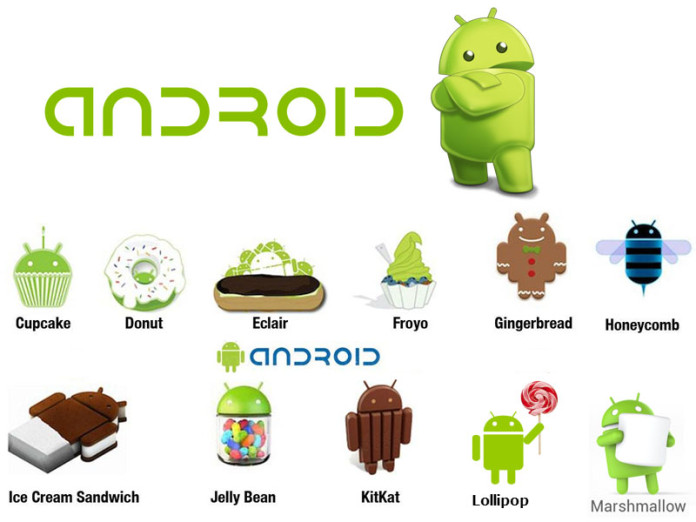
\includegraphics[scale=.4]{android_version.jpg}
    \end{center}
    \caption{Các phiên bản của hệ điều hành Android tính đến thời điểm hiện tại}
    \label{refhinh1}
    \end{figure}
\end{center}
Android có mã nguồn mở và Google phát hành mã nguồn theo Giấy phép Apache. Chính mã nguồn mở cùng với một giấy phép không có nhiều ràng buộc đã cho phép các nhà phát triển thiết bị, mạng di động và các lập trình viên nhiệt huyết được điều chỉnh và phân phối Android một cách tự do. Ngoài ra, Android còn có một cộng đồng lập trình viên đông đảo chuyên viết các ứng dụng để mở rộng chức năng của thiết bị, bằng một loại ngôn ngữ lập trình Java có sửa đổi. Chính vì vây, Android có một tốc độ mở rộng và phát triển không tưởng, chiếm thị phần lớn nhất trong hệ thống điện thoại thông minh toàn cầu (84.1\% vào quý 1 năm 2016) \cite{bib6} (Hình 14)
\begin{center}
    \begin{figure}[h]
    \begin{center}
     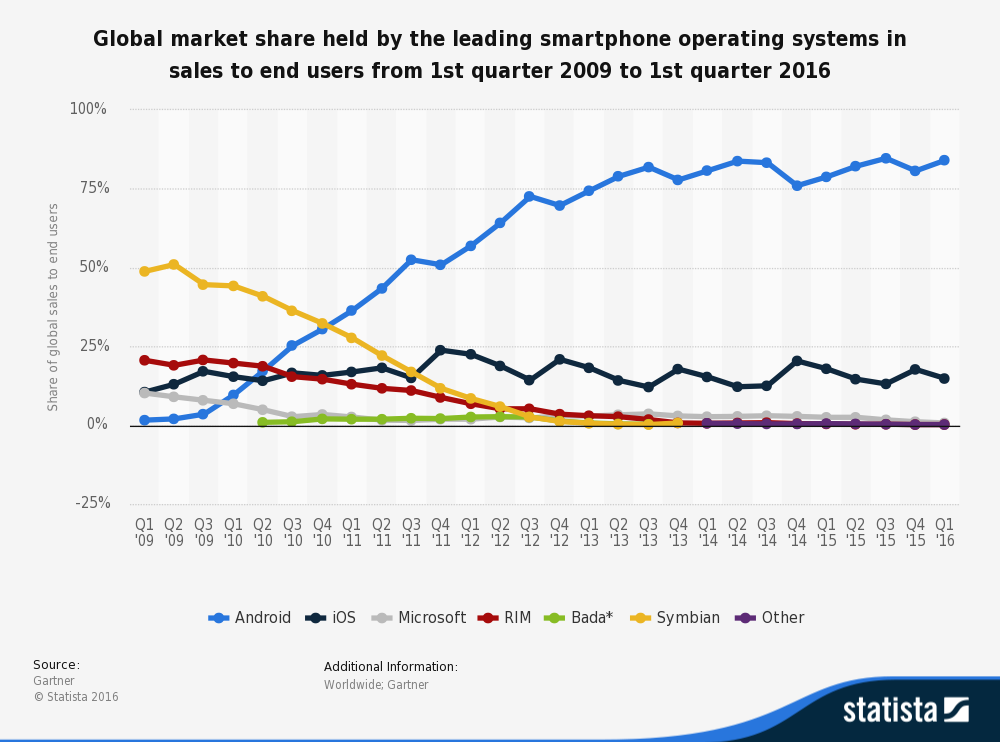
\includegraphics[scale=.25]{android_shipment_market.png}
    \end{center}
    \caption{Thị phần điện thoại thông minh phân loại theo hệ điều hành}
    \label{refhinh1}
    \end{figure}
\end{center}
Vào tháng 2 năm 2016, có khoảng 2 triệu ứng dụng trên Android \cite{bib7}, và số lượt tải ứng dụng từ Google Play, cửa hàng ứng dụng chính của Android, ước tính khoảng 65 tỉ lượt tải \cite{bib8} (Hình 16)
\begin{figure}[h]
\centering
\begin{subfigure}{.5\textwidth}
  \centering
  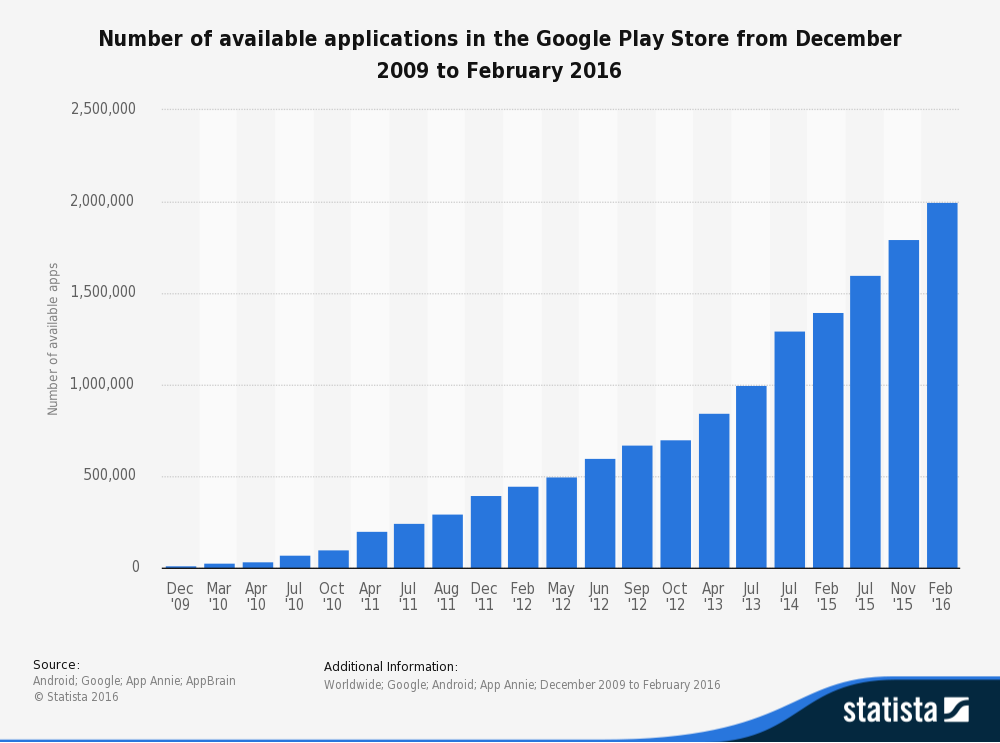
\includegraphics[width=0.95\linewidth]{number_app.png}
  \caption{Số ứng dụng trên Android}
\end{subfigure}%
\begin{subfigure}{.5\textwidth}
  \centering
  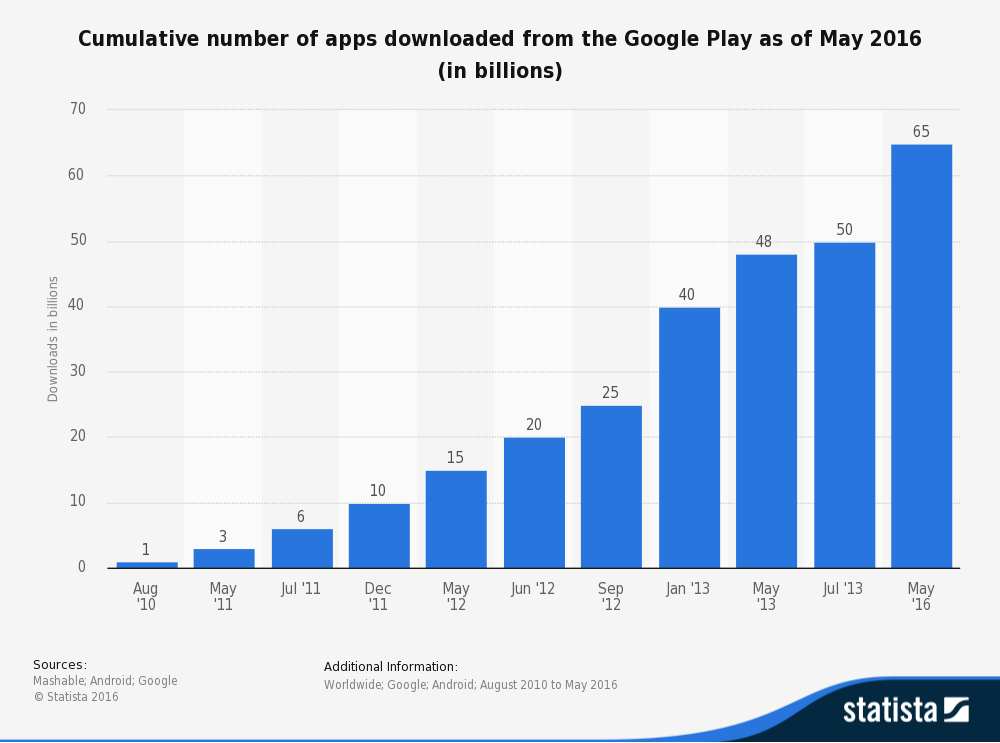
\includegraphics[width=0.95\linewidth]{number_app_downloads.PNG}
  \caption{Số lượt tải ứng dụng trên Android}
  \label{fig:sub2}
\end{subfigure}
\caption{Số lượt tải và số lượng ứng dụng Android giai đoạn 2009-2016}
\end{figure} 
\subsubsection{Nguyên nhân sự phát triển mạnh mẽ của Android}
\begin{itemize}
	\item[•] \textbf{Mã nguồn mở:} Bởi vì Android là mã nguồn mở nên lập trình viên dễ dàng tiếp cận với Android và thử nghiệm các công nghệ mới vào Android.
	\item[•] \textbf{Mở rộng tầm ảnh hưởng của cộng đồng và lập trình viên}
	\item[•] \textbf{Tăng hiệu quả marketing:} Dựa vào sự hỗ trợ từ Google Play, marketing cho ứng dụng trên Android có nhiều lợi thế hơn, dễ dàng quảng cáo ứng dụng đến người dùng trên toàn cầu.
	\item[•] \textbf{Kết hợp các ứng dụng:} Android có tính linh động cao và có hỗ trợ để kết hợp với các ứng dụng trên các nền tảng khác.
	\item[•] \textbf{Giảm chi phí phát triển: }Các công cụ để lập trình Android hoàn toàn miễn phí, và Google chỉ thu một khoản phí nhỏ để đưa ứng dụng Android lên Android Market. Việc xây dựng và phát triển một ứng dụng Android gần như không tốn chi phí.
	\item[•] \textbf{Tỉ lệ thành công cao.}
	\item[•] \textbf{Môi trường lập trình tốt:} Android cung cấp nhiều công cụ hỗ trợ tốt, SDK và các công nghệ hấp dẫn với lập trình viên để giúp họ sử dụng và phát triển ứng dụng.
\end{itemize}
\subsubsection{Các tính năng cơ bản của Android}
Android là một hệ điều hành đầy sức mạnh và hỗ trợ nhiều tính năng tuyệt vời, danh sách các tính năng cơ bản của Android được nhóm liệt kê trong Bảng 1.
\begin{table}[h]
\centering
\begin{tabular}{|l|l|}
\hline
\rowcolor[HTML]{C0C0C0} 
\textbf{Đặc điểm}& \textbf{Miêu tả} \\
\hline
Giao diện đẹp 	 & Màn hình Android OS cơ bản cung cấp một giao diện người dùng đẹp \\
			  	 & và có tính thẩm mỹ cao \\ \hline
Tính kết nối  	 & GSM/EDGE, IDEN, CDMA, EV-DO, UMTS, Bluetooth, Wi-Fi, LTE, \\ 
			  	 & NFC và WiMAX \\ 
\hline
Lưu trữ 	  	 & SQLite, một cơ sở dữ liệu quan hệ gọn nhẹ, được sử dụng cho mục đích \\ 
			  	 & lưu trữ dữ liệu \\
\hline
Hỗ trợ Media 	 & H.263, H.264, MPEG-4 SP, AMR, AMR-WB, AAC, HE-AAC, AAC 5.1, \\ 
			  	 & MP3, MIDI, Ogg Vorbis, WAV, JPEG, PNG, GIF, và BMP \\
\hline
Tin nhắn 	  	 & SMS và MMS \\
\hline
Trình duyệt Web  & Dựa trên thiết bị WebKit mã nguồn mở, đi kèm với thiết bị V8  \\ 
				 & JavaScript của Chrome hỗ trợ HTML5 và CSS3 \\
\hline
Multi-touch 	 & Android hỗ trợ cho multi-touch mà đã được tạo ban đầu có sẵn cho \\ 
				 & các Handset \\
 \hline
Đa nhiệm 		 & Người dùng có thể nhảy từ một tác vụ tới tác vụ khác và nhiều ứng\\ 
				 & dụng có thể chạy đồng thời cùng một lúc \\
\hline
Widget tùy chỉnh & Widgets có thể thay đổi kích cỡ, vì thế người dùng có thể mở rộng để\\ 
				 & hiển thị nhiều nội dung hơn, hoặc thu nhỏ để tiết kiệm không gian\\
\hline
Đa ngôn ngữ 	 & Hỗ trợ text đơn hướng và song hướng \\
\hline
GCM 			 & Google Cloud Messaging (GCM) là một dịch vụ cho phép lập trình viên\\ 
				 & gửi thông điệp dữ liệu ngắn tới người dùng trên thiết bị Android, mà  \\
				 & không cần một Sync Solution \\
\hline
Wi-Fi Direct 	 & Một công nghệ cho phép các ứng dụng dò tìm và ghép cặp một cách \\ 
				 & trực tiếp, thông qua một kết nối peer-to-peer \\
\hline
Android Beam 	 & Một công nghệ dựa trên NFC phổ biến cho phép người dùng chia sẻ tức \\ 
				 & thì, chỉ cần kích hoạt NFC của hai điện thoại với nhau \\
\hline
\end{tabular}
\caption{Các tính năng cơ bản của hệ điều hành Android}
\label{my-label}
\end{table}
%%%%%%%%%%%%%%%%%%%%%%%%%%%%%%%%%
\section{Hiện thực dự án}
Với các kiến thức nền như trên và các phân tích về yêu cầu của đề tài, nhóm xin sử dụng các công nghệ trong phần kiến thức nền để hiện thực đề tài.
\subsection{Cơ sở dữ liệu}
Từ những phân tích về các chức năng của ứng dụng, nhóm xác định cơ sở dữ liệu sẽ bao gồm bảng User quản lý các tài khoản và thông tin người dùng, bảng Request và Comment lưu trữ góp ý và bình luận của người dùng. Lược đồ Entity - Relationship giữa các thực thể trong ứng dụng được mô tả ở Hình 16, bao gồm:
\begin{itemize}
\item[•]\textbf{Request: }Là thực thể mô tả một góp ý của người dân đến chính quyền, các thuộc tính của thực thể này bao gồm tên, mã số, địa chỉ, mô tả, hình ảnh, vị trí, id người gửi, v.v
\item[•]\textbf{Comment: }Là thực thể mô tả bình luận trong về một góp ý nào đó, có thể có nhiều bình luận trong một góp ý, các thuộc tính của thực thể bao gồm id của bình luận, thời gian gửi, nội dung và thông tin người gửi
\item[•]\textbf{User: }Là thực thể chứa thông tin của một người dùng, đây là thực thể tổng quát hóa, bao gồm hai thực thể con là \textit{người dùng thông thường (normal user)} và \textit{khách (guest).} Các thuộc tính của thực thể này bao gồm id, loại người dùng, email, tên và token của tài khoản
\item[•]\textbf{Normal User: }Là thực thể chứa thông tin của người dùng thông thường, được thừa kế từ thưc thể User, bao gồm các thuộc tính id, số CMND, mật khẩu và số điện thoại
\item[•]\textbf{Guest User: }Là thực thể chứa thông tin của khách, được thừa kế từ thực thể User, chỉ có một thuộc tính là id
\end{itemize}
Tuy nhiên nhóm không tạo trước cơ sở dữ liệu mà sử dụng chức năng tạo ra cơ sở dữ liệu động trong lần chạy đầu tiên của ứng dụng. Việc này được thực hiện thông qua JPA API, các bảng trong cơ sở dữ liệu tương ứng với các JPA Entity đã được hiện thực trước đó.\\
\\
Lược đồ class của dự án được thể hiện ở Hình 17.
\begin{center}
    \begin{figure}[h]
    \begin{center}
     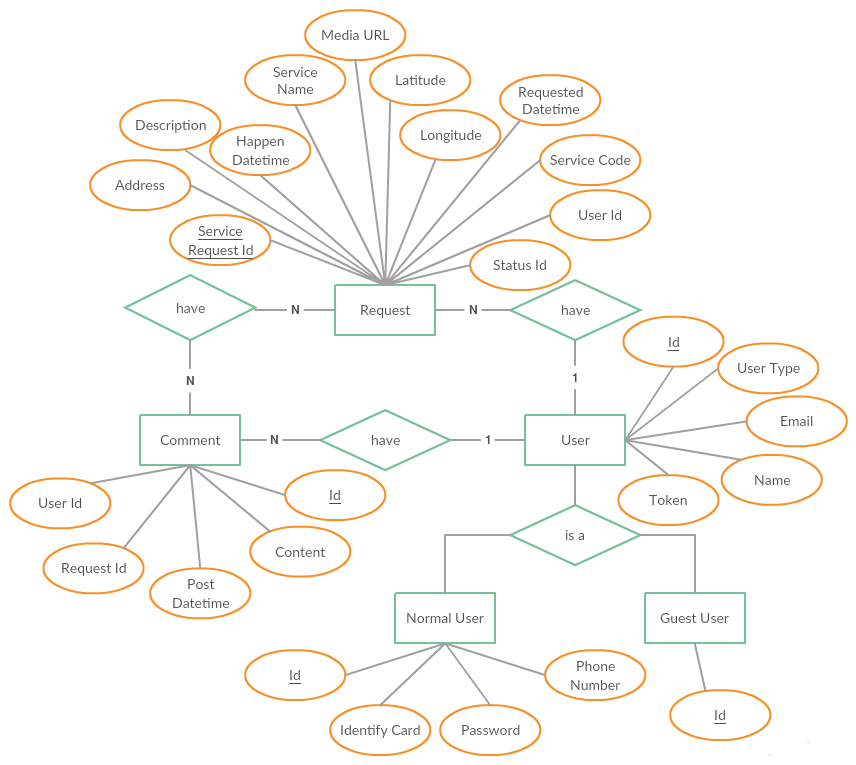
\includegraphics[scale=.65]{entity-diagram.png}
    \end{center}
    \caption{Mô hình Entity - Relationship của đề án}
    \label{refhinh1}
    \end{figure}
\end{center}

\newpage
\begin{center}
    \begin{figure}[h]
    \begin{center}
     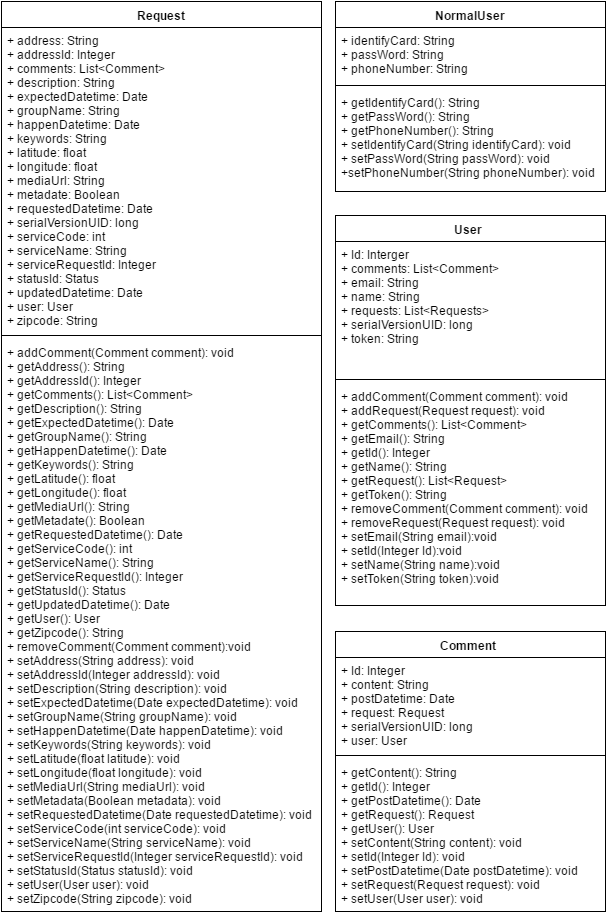
\includegraphics[scale=.6]{class-diagram.png}
    \end{center}
    \caption{Mô hình Class Diagram của đề án}
    \label{refhinh1}
    \end{figure}
\end{center}
\newpage
\subsection{Web Service}
Với từng thực thể nói trên, nhóm đã hiện thực các Web Service tương ứng:
\subsubsection*{Request}
    \begin{center}
        \begin{table}[h]
            \begin{tabular}{|l|l|l|m{7.2cm}|}
            \hline
            \rowcolor[HTML]{C0C0C0} 
            \textbf{Tên} & \textbf{Phương thức} & \textbf{Đối số} & \textbf{Mô tả}\\
            \hline
            find & GET & id của Request & Lấy thông tin của một thực thể Request theo \\
            	&&&id\\ 
            \hline
            findAll & GET &   & Lấy thông tin của mọi Request có trong cơ sở \\
            &&&dữ liệu\\
            \hline
            create & POST & Request mới  & Thêm một Request mới vào cơ sở dữ liệu\\          
            \hline
            edit & PUT & - id của Request  & Cập nhật một Request theo id của nó\\
            && - Request mới & \\
            \hline        
            remove & DELETE & id của Request  & Xóa một Request theo id\\            
            \hline                    
            \end{tabular}
        \end{table}    
    \end{center}
\subsubsection*{Comment}
    \begin{center}
        \begin{table}[h]
            \begin{tabular}{|l|l|l|m{5.0cm}|}
            \hline
            \rowcolor[HTML]{C0C0C0} 
            \textbf{Tên} & \textbf{Phương thức} & \textbf{Đối số} & \textbf{Mô tả}\\
            \hline
            find & GET & id của Comment & \pbox{24cm}{Lấy thông tin của một thực thể\\ Comment theo id}\\ [5pt]    
            \hline
            findAll & GET & \  & \pbox{24cm}{Lấy thông tin của mọi Comment \\có trong cơ sở dữ liệu}\\[5pt]    
            \hline
            findAllByRequestId & GET & id của Request  & \pbox{24cm}{Lấy thông tin mọi Comment \\ trong một Request theo id \\của Request}\\       [5pt]         
            \hline
            create & POST & Comment mới  & \pbox{24cm}{Thêm một Comment mới vào cơ \\sở dữ liệu}\\[5pt]            
            \hline
            edit & PUT & \pbox{24cm}{- id của Comment \\ - Comment mới}  & \pbox{24cm}{Cập nhật một Comment theo id \\của nó}\\ [5pt]             
            \hline        
            remove & DELETE & \pbox{24cm}{id của Comment}  & \pbox{24cm}{Xóa một Comment theo id}\\ [5pt]              
            \hline                    
            \end{tabular}
        \end{table}    
    \end{center}
    \newpage
\subsubsection*{GuestUser}
    \begin{center}
        \begin{table}[h]
            \begin{tabular}{|l|l|l|m{7.6cm}|}
            \hline
            \rowcolor[HTML]{C0C0C0} 
            \textbf{Tên} & \textbf{Phương thức} & \textbf{Đối số} & \textbf{Mô tả}\\
            \hline
            create & POST & GuestUser mới  & \pbox{24cm}{Thêm một GuestUser mới vào cơ sở dữ liệu}\\[5pt]            
            \hline                    
            \end{tabular}
        \end{table}    
    \end{center}

\subsubsection*{NormalUser}
    \begin{center}
        \begin{table}[h]
            \begin{tabular}{|l|l|l|m{6.6cm}|}
            \hline
            \rowcolor[HTML]{C0C0C0} 
            \textbf{Tên} & \textbf{Phương thức} & \textbf{Đối số} & \textbf{Mô tả}\\
            \hline
            find & GET & id của NormalUser & \pbox{24cm}{Lấy thông tin của một thực thể NormalUser\\ theo id}\\ [5pt]
            \hline
            findAll & GET & \  & \pbox{24cm}{Lấy thông tin của mọi NormalUser có trong\\ cơ sở dữ liệu}\\[5pt]
            \hline
            create & POST & NormalUser mới  & \pbox{24cm}{Thêm một NormalUser mới vào cơ sở dữ \\liệu}\\[5pt]            
            \hline
            edit & PUT & \pbox{24cm}{- id của NormalUser \\ - NormalUser mới}  & \pbox{24cm}{Cập nhật một NormalUser theo id của nó}\\[5pt]            
            \hline        
            remove & DELETE & \pbox{24cm}{id của NormalUser}  & \pbox{24cm}{Xóa một NormalUser theo id}\\[5pt]            
            \hline                    
            \end{tabular}
        \end{table}    
    \end{center}
\subsubsection*{Xác thực}
Để quản lý quá trình xác thực người dùng khi đăng nhập, nhóm đã hiện thực thêm một Web Service có chức năng xác thực người dùng:
    \begin{center}
        \begin{table}[h]
            \begin{tabular}{|l|l|l|m{6.3cm}|}
            \hline
            \rowcolor[HTML]{C0C0C0} 
            \textbf{Tên} & \textbf{Phương thức} & \textbf{Đối số} & \textbf{Mô tả}\\
            \hline
            authenticationUser & POST & \pbox{24cm}{- email \\ - password}  & \pbox{24cm}{Xác thực người dùng theo email và \\password}\\[5pt]            
            \hline                    
            \end{tabular}
        \end{table}    
    \end{center}
\subsection{Client}
Trong giai đoạn TTTN, nhóm đang hiện thực dự án trên nền tảng web. Từ các yêu cầu đã được nhóm tìm hiểu ở những mục trên, nhóm đã hiện thực được các trang giao diện sau:
\newpage
\begin{itemize}
	\item[•]Trang list-issue (Hình 18): Trang danh sách phản ánh cũng là trang chủ của hệ thống. Các phản ánh sẽ được hiển thị tại đây dưới dạng danh sách, cùng với đó là các bình luận dành cho mỗi phản ánh, phía bên trái là bản đồ hiển thị vị trí các phản ánh.
	\begin{center}
    	\begin{figure}[h]
    	\begin{center}
    	 	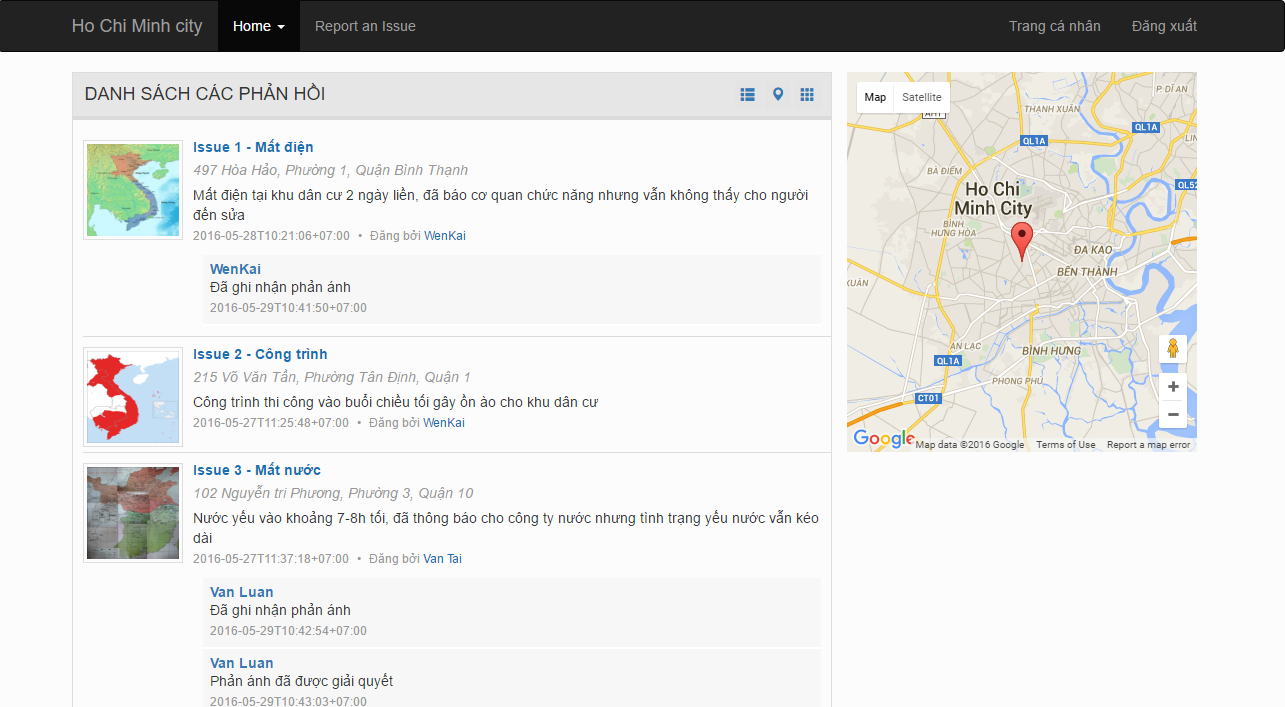
\includegraphics[scale=.35]{list-issue.PNG}
    	\end{center}
    	\caption{Trang list-issue}
    	\label{refhinh1}
    	\end{figure}
    \end{center}
	\item[•]Trang map-issue (Hình 19): Hiển thị bản đồ vị trí các phản ánh một cách chi tiết hơn. Phía bên trái là danh sách thu gọn các phản ánh.
    
\begin{center}
    	\begin{figure}[h]
    	\begin{center}
    	 	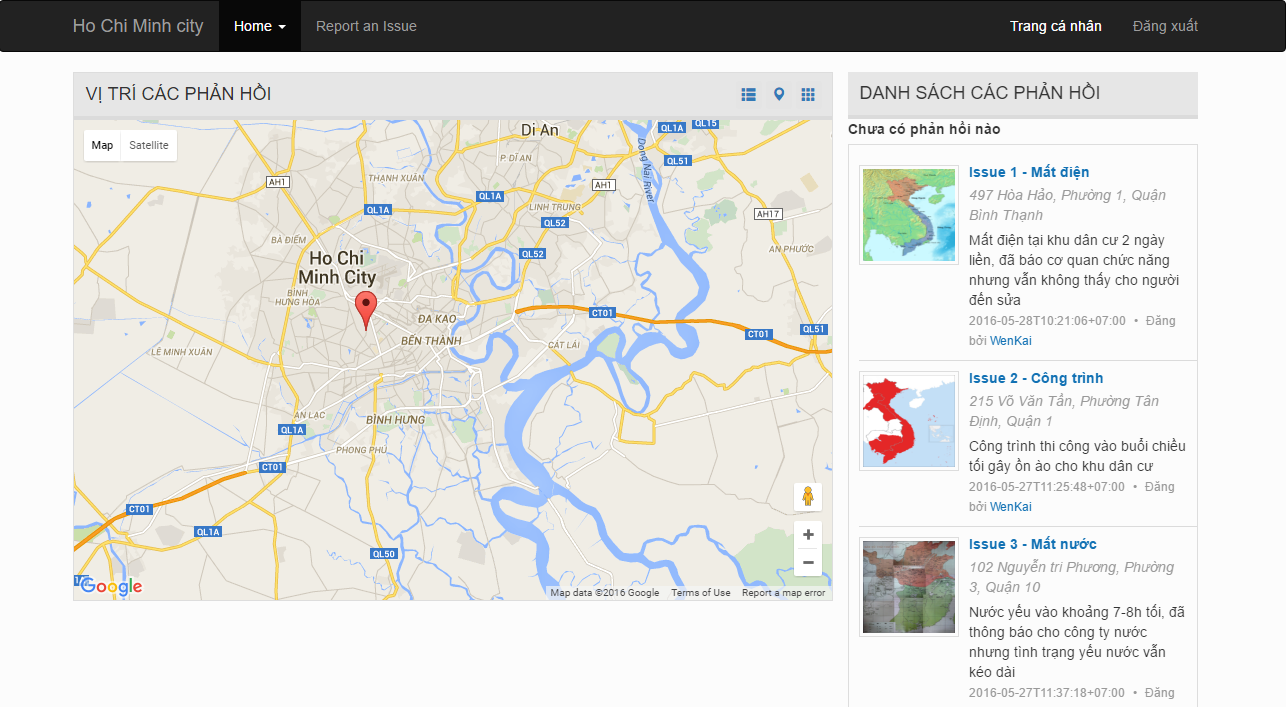
\includegraphics[scale=.35]{map-issue.PNG}
    	\end{center}
    	\caption{Trang map-issue}
    	\label{refhinh1}
    	\end{figure}
    \end{center}	
    \newpage
	\item[•]Trang gallery-issue (Hình 20): Hiển thị danh sách các phản ánh theo dạng danh sách ảnh. Phía bên trái là danh sách thu gọn các phản ánh.
\begin{center}
    	\begin{figure}[htp]
    	\begin{center}
    	 	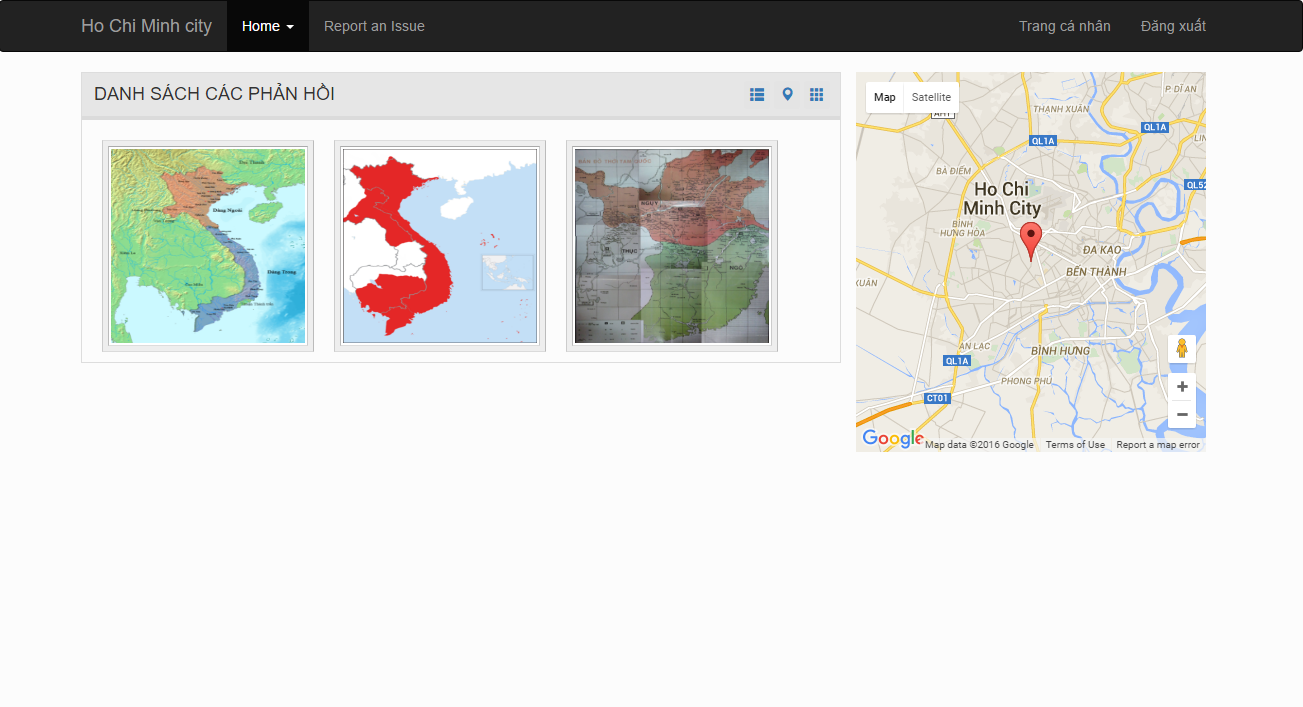
\includegraphics[scale=.35]{gallery-issue.PNG}
    	\end{center}
    	\caption{Trang gallery-issue}
    	\label{refhinh1}
    	\end{figure}
    \end{center}	
	\item[•]Trang issue-detail (Hình 21): Hiển thị chi tiết về một phản ánh, người dùng cũng có thể đăng bình luận về phẩn ánh đó.
\begin{center}
    	\begin{figure}[htp]
    	\begin{center}
    	 	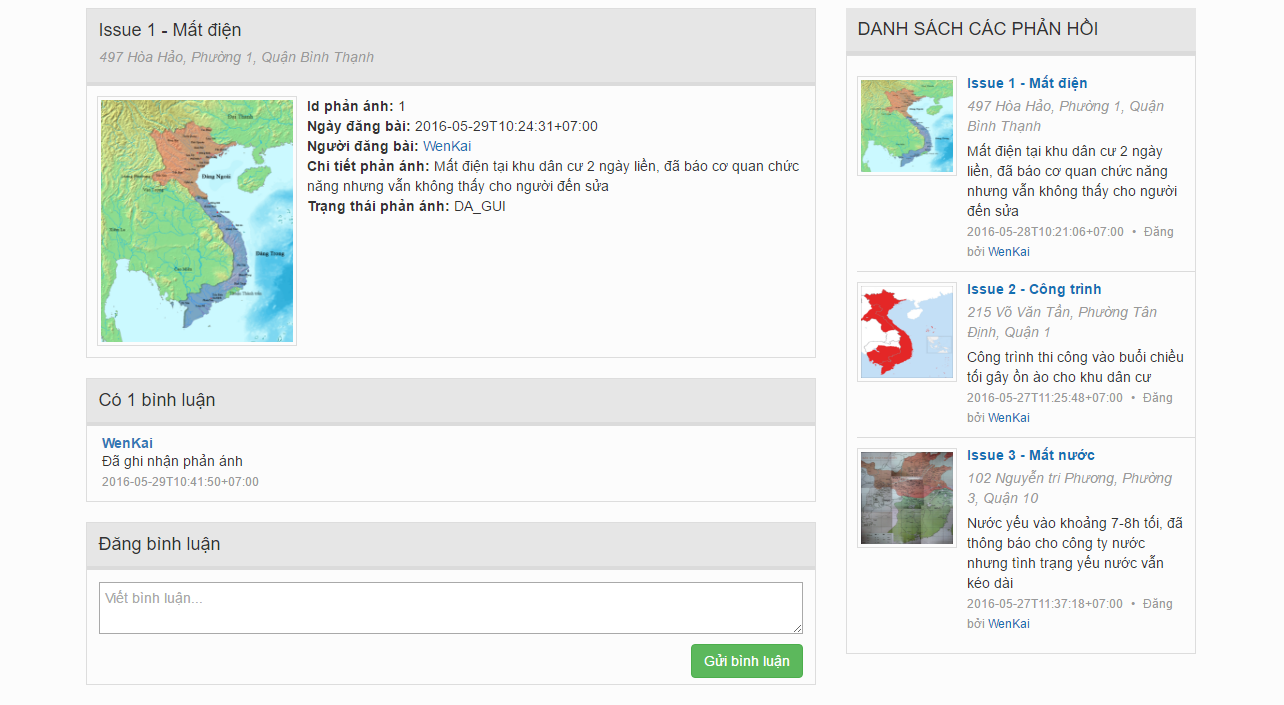
\includegraphics[scale=.35]{issue-detail.PNG}
    	\end{center}
    	\caption{Trang issue-detail}
    	\label{refhinh1}
    	\end{figure}
    \end{center}
    \newpage
	\item[•]Trang report-issue (Hình 22): Cho phép người dùng đăng lên một phản ánh, trang này được chia làm bốn bước khác nhau giúp người dùng dễ dàng hơn trong việc cung cấp thông tin về phản ánh.
\begin{figure}[h]
		\centering
		\begin{subfigure}{.5\textwidth}
  			\centering
  			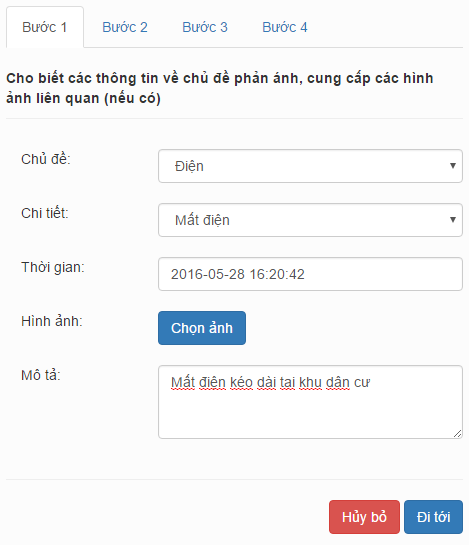
\includegraphics[width=0.6\linewidth]{Step1.PNG}
 		    \caption{}
		\end{subfigure}%
		\begin{subfigure}{.5\textwidth}
  			\centering
  			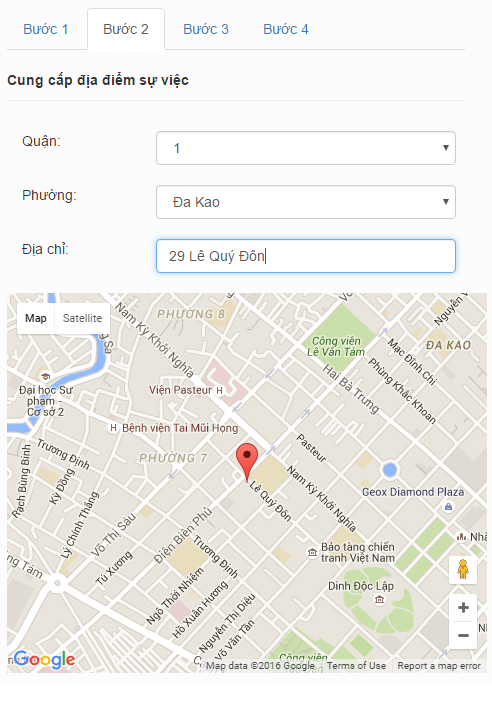
\includegraphics[width=0.6\linewidth]{Step2.PNG}
  			\caption{}
  			\label{fig:sub2}
		\end{subfigure}
		\begin{subfigure}{.5\textwidth}
  			\centering
  			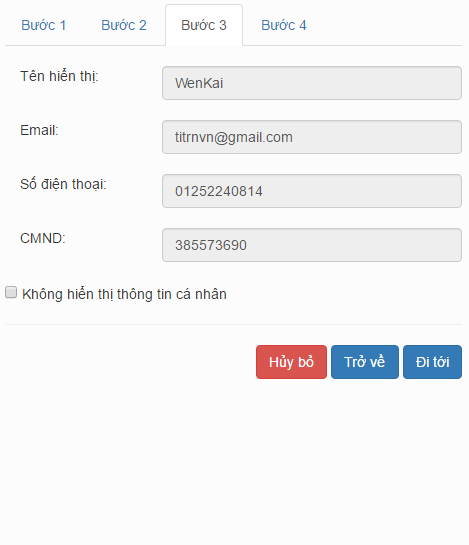
\includegraphics[width=0.6\linewidth]{Step3.PNG}
  			\caption{}
  			\label{fig:sub2}
		\end{subfigure}%
		\begin{subfigure}{.5\textwidth}
  			\centering
  			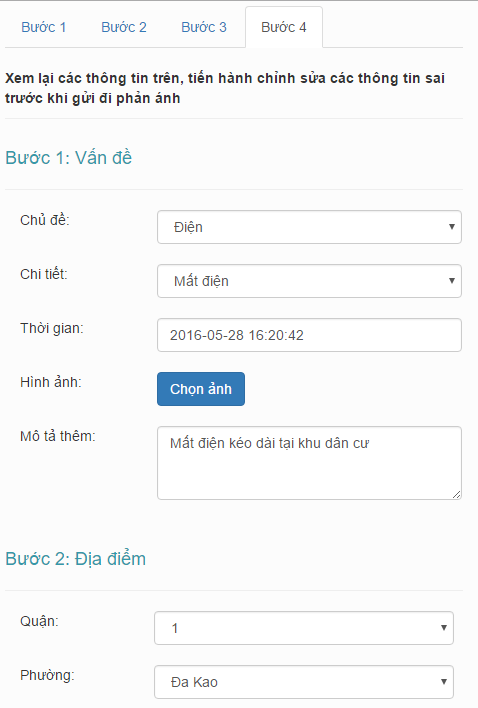
\includegraphics[width=0.6\linewidth]{Step4.PNG}
  			\caption{}
  			\label{fig:sub2}
		\end{subfigure}
		\caption{Trang report-issue}
	\end{figure}
\end{itemize}


    

    

    

	\newpage
	

\section{Khó khăn và thách thức}
Ở Việt Nam, CPĐT là một cơ hội lớn để cải cách cách thức làm việc của bộ máy nhà nước, nâng cao hiệu suất và chất lượng; đồng thời giúp người dân tương tác với các dịch vụ nhà nước dễ dàng. Tuy vậy, CPĐT cũng tồn tại nhiều thách thức cần vượt qua trong quá trình triển khai ở Việt Nam. Ở phần này, nhóm xin trình bày một số thách thức trong việc triển khai CPĐT trên lĩnh vực công nghệ.
\subsection{Hạ tầng công nghệ thông tin và truyền thông}
Hạ tầng công nghệ thông tin và truyền thông là một trong những thách thức lớn nhất trong quá trình hiện thực CPĐT. Công nghệ thông tin và truyền thông, gọi tắt là ICT, bao gồm tất cả các phương tiện kỹ thuật được sử dụng để xử lý thông tin và trợ giúp liên lạc như: phần cứng, mạng máy tính, các phần mềm cần thiết, điện thoại, và phương tiện truyền thông. Để chuyển đổi sang CPĐT, cần có hạ tầng công nghê thông tin theo các chuẩn và mô hình cần thiết đảm bảo cho việc chuyển đổi. Chỉ số phát triển ICT ở Việt Nam còn thấp (4.26 vào năm 2015, xếp hạng 102 trên thế giới \cite{bib9}) và tình trạng hạ tầng công nghệ thông tin và truyền thông không đồng đều, chỉ phát triển chủ yếu ở các thành phố lớn cho thấy khó khăn trong việc triển khai CPĐT ở Việt Nam.
\subsection{Bảo mật}
Thực tế cho thấy bảo mật là một trong những thách thức quan trọng nhất trong quá trình hiện thực CPĐT. Bảo mật có nghĩa bảo vệ mọi thông tin và hệ thống, tránh khỏi các truy cập vượt quyền, các thay đổi trái phép lên hệ thống hoặc các cuộc tấn công phá hủy hệ thống. Vì vậy, bảo mật liên quan đến việc bảo vệ hệ thống thông tin, quản lý quyền truy cập thông tin. Đó là thành phần không thể thiếu để xây dựng CPĐT, tạo nên mối quan hệ tin tưởng giữa người dân và chính phủ.\\
\\
Một số giải pháp có thể được sử dụng để bảo mật như: chữ ký số, mã hóa, sử dụng tên đăng nhập, mật khẩu và một số biện pháp khác có thể giải quyết vấn đề bảo mật trong các ứng dụng CPĐT.
\subsection{Tính riêng tư}
Một trở ngại then chốt trong việc hiện thực CPĐT là phải đảm bảo tính riêng tư về cuộc sống của người dân và bí mật các thông tin cá nhân. Chính phủ cần sử dụng các biện pháp công nghệ phù hợp để bảo vệ sự riêng tư cá nhân, bởi vì chỉ có đảm bảo quyền riêng tư cá nhân mới khiến người dân cảm thấy tự tin khi sử dụng các dịch vụ của CPĐT.
\subsection{Tương tác đa chiều}
Một ứng dụng CPĐT thật sự hiệu quả khi người dân có thể truy cập thông qua nhiều thiết bị, phương thức khác nhau. Chính vì vậy, cần phát triển ứng dụng CPĐT trên nhiều nền tảng khác nhau, như là nền tảng Web và di động.

%%%%%%%%%%%%%%%%%%%%%%%%%%%%%%%%%
\section{Mở rộng đề tài}
Hiện tại nhóm chỉ mới phát triển ứng dụng trên nền Web. \\ 
\\
Trong giai đoạn luận văn tốt nghiệp, nhóm sẽ hoàn thành các nhiệm vụ sau:
\begin{itemize}
	\item[•]Hoàn chỉnh giao diện web cho ứng dụng
	\item[•]Tiếp tục tìm hiểu về cách làm việc của CPĐT, thủ tục hành chính của các bên liên quan để hoàn thiện các luồng làm việc của ứng dụng
	\item[•]Sửa chữa các lỗi còn tồn tại
	\item[•]Phát triển ứng dụng trên nền tảng di động
	\item[•]Viết báo cáo về đề tài
\end{itemize}
%%%%%%%%%%%%%%%%%%%%%%%%%%%%%%%%%
\section{Kết luận}
Đề án Chính phủ điện tử hiện nay là cơ hội lớn cho ngành công nghệ thông tin Việt Nam. Nhận thấy tầm quan trọng của nó, hy vọng với đề tài này, nhóm có thể góp sức vào công cuộc phát triển và áp dụng CPĐT vào thực tiễn ở địa bàn Thành phố Hồ Chí Minh \\
\\
Sau cuối, nhóm xin cảm ơn thầy Lương Thế Nhân đã hỗ trợ giải đáp các khó khăn và vướng mắc, giúp đỡ nhóm trong quá trình hiện thực đề tài.

\newpage
\section{Phụ lục}
\begin{thebibliography}{99}
\bibitem{bib1}
United Nation (13/01/2010). \textit{A General Framework for E-Government: Definition - Maturity Challenges, Opportunities, and Success.} Truy cập 18/05/2016 tại \url{http://www.unpan.org/Library/MajorPublications/UNEGovernmentSurvey/PublicEGovernanceSurveyintheNews/tabid/651/mctl/ArticleView/ModuleId/1555/articleId/20840/Default.aspx}

\bibitem{bib2}
World Bank (19/05/2015). \textit{Information \& Communication Technologies: e-Government.} Truy cập 18/05/2016 tại \url{http://www.worldbank.org/en/topic/ict/brief/e-government}

\bibitem{bib3}
United Nation (2014). \textit{Data Center: 2014 E-Government Development Index.} Truy cập 18/05/2016 tại \url{https://publicadministration.un.org/egovkb/en-us/Data-Center}

\bibitem{bib33}
Ministry of Finance Singapore (4/9/2013). \textit{E-Government in Singapore.} Truy cập 23/05/2016 tại \url{http://workspace.unpan.org/sites/Internet/Documents/UNPAN90601.pdf}

\bibitem{bib4}
Open311 Documents. Truy cập 22/05/2016 tại
 \url{http://www.open311.org/} 
 
 \bibitem{bib11}
RESTful Web services: The basics. Truy cập 22/05/2016 tại
 \url{https://www.ibm.com/developerworks/library/ws-restful/} 
 
 \bibitem{bib12}
Tổng quát về JPA (Java Persistence API). Truy cập 22/05/2016 tại
 \url{http://linkit.vn/tong-quat-ve-jpa-java-persistence-api-3355720.htm} 
 
 \bibitem{bib5}
AngularJS Documents. Truy cập 22/05/2016 tại
 \url{https://docs.angularjs.org/} 
 
  \bibitem{bib6}
Thị phần điện thoại thông minh. Truy cập 22/05/2016 tại
 \url{http://www.statista.com/statistics/266136/global-market-share-held-by-smartphone-operating-systems/} 

  \bibitem{bib7}
Số lượng ứng dụng trên Android. Truy cập 22/05/2016 tại
 \url{http://www.statista.com/statistics/266210/number-of-available-applications-in-the-google-play-store/}
 
   \bibitem{bib8}
Số lần tải ứng dụng trên Android. Truy cập 22/05/2016 tại
 \url{http://www.statista.com/statistics/281106/number-of-android-app-downloads-from-google-play/}

   \bibitem{bib9}
Chỉ số phát triển ICT ở Việt Nam năm 2015
 \url{https://www.itu.int/net4/ITU-D/idi/2015/}
 
\bibitem{bib10}
M. Alshehri, S. Drew , 2010. \textit{Implementation of e-Government:
Advantages and Challenges}. Truy cập tại \url{http://www98.griffith.edu.au/dspace/bitstream/handle/10072/40620/72631_1.pdf?sequence=1.}.

%\bibitem{}
%Tên tác giả, năm xuất bản. \textit{Tên sách.} Lần xuất bản. Thành phố: Nhà xuất bản.

\end{thebibliography}

\newpage
\section*{Đánh giá mức độ đóng góp}
        \begin{table}[h]
        \centering
            \begin{tabular}{|l|l|l|}
            \hline
            STT & Tên & Mức độ đóng góp\\
            \hline
            1 & Võ Văn Luận & 50\%\\
            \hline
            2 & Trần Văn Tài & 50\%\\           
            \hline
            \end{tabular}
        \end{table}  

\listoffigures
\newpage
%%%%%%%%%%%%%%%%%%%%%%%%%%%%%%%%%

\end{document}

